\documentclass[11pt]{article}
\usepackage[final]{acl}

\usepackage{times}
\usepackage{latexsym}
\usepackage[T1]{fontenc}
\usepackage[utf8]{inputenc}
\usepackage{microtype}
\usepackage{graphicx}
\usepackage{booktabs}
\usepackage{amsmath}
\usepackage{amssymb}
\usepackage{amsthm}
\usepackage{enumitem}
\usepackage{multirow}
\usepackage{xspace}
\usepackage{array}
\usepackage{tikz}
\usetikzlibrary{shapes,arrows,positioning,calc}
\usepackage{algorithm}
\usepackage{algpseudocode}
\renewcommand{\algorithmicrequire}{\textbf{Input:}}
\renewcommand{\algorithmicensure}{\textbf{Output:}}

\newcommand{\system}{\textsc{EVIRAG}\xspace}
\newcommand{\bench}{\textsc{EVIRAG-Bench}\xspace}
\setlength\titlebox{6.3cm}

\newtheorem{definition}{Definition}
\newtheorem{proposition}{Proposition}
\newtheorem{remark}{Remark}

%% ─────────────────────────────────────────────────────────────────────────────
\hypersetup{
  pdftitle={Beyond Epistemic Collapse: Disagreement-Aware Scientific
            Retrieval-Augmented Generation},
  pdfauthor={Animesh Mishra, Krishang Sharma, Sonia Khetarpaul},
  pdfsubject={EMNLP 2026},
  pdfkeywords={retrieval-augmented generation, scientific QA, disagreement,
               epistemic collapse, viewpoint coverage}
}

\title{Beyond Epistemic Collapse: Disagreement-Aware Scientific\\
       Retrieval-Augmented Generation}

\author{
  Animesh Mishra\textsuperscript{1} \quad
  Krishang Sharma\textsuperscript{2} \quad
  Sonia Khetarpaul\textsuperscript{2} \\
  \textsuperscript{1}Indian Institute of Technology Patna, India \\
  \textsuperscript{2}Department of Computer Science and Engineering, \\
  Shiv Nadar Institution of Eminence, Delhi-NCR, India \\
  \texttt{animesh\_ua2501bbh143@iitp.ac.in} \\
  \texttt{ks243@snu.edu.in} \quad
  \texttt{sonia.khetarpaul@snu.edu.in}
}

\begin{document}
\maketitle

%% ─────────────────────────────────────────────────────────────────────────────
\begin{abstract}
Scientific retrieval-augmented generation (RAG) systems typically return one
fluent answer even when the underlying literature contains multiple
well-supported but incompatible views.  We call this failure mode
\emph{epistemic collapse}: compression of structured disagreement into a single
response.  We present \system\ (Evidence-centric, Viewpoint-Inclusive RAG), a
framework for scientific question answering that combines adversarial retrieval,
claim-level disagreement graphs, causal disagreement attribution, multi-view
synthesis, and evidence-structured confidence labels.  We also introduce
\bench, a 1,250-query benchmark spanning five contested scientific domains.
Across eight systems and three controls, \system\ substantially outperforms
vanilla RAG on ContradictionRecall and dense-encoder ViewpointCoverage while
reducing Single-View Concentration.  A single-call structured-prompt baseline
recovers most of the viewpoint-coverage gap but only about a quarter of the
contradiction-recall gap, isolating what the claim graph contributes beyond
output formatting.  Human evaluation with three annotators confirms markedly
higher epistemic completeness for \system\ (Krippendorff's $\alpha{=}0.72$,
$p{<}0.001$, Cohen's $d{=}2.71$), an ordering that survives censoring the
rubric at its second-highest anchor.  An offline precomputed graph reduces
warm-query latency by over an order of magnitude.  These results support
treating disagreement preservation as a primary design objective for
disagreement-heavy scientific QA.
\end{abstract}

%% ─────────────────────────────────────────────────────────────────────────────
\section{Introduction}
\label{sec:intro}

Scientific question answering has advanced rapidly through retrieval-augmented
generation (RAG), which grounds model responses in retrieved
documents~\citep{lewis2020rag}.  Yet a fundamental challenge remains: when the
literature is genuinely contested, what should a responsible system return?
Current architectures optimize for a single coherent answer---a design suited
to lookup queries but structurally misaligned with contested knowledge, where
authoritative sources support mutually incompatible conclusions.  Questions
such as \textit{Does homework improve achievement?}
\citep{cooper2006homework,masalimova2023science,scheb2023hurt},
\textit{Do statins help in primary
prevention?}~\citep{ridker2008jupiter}, or \textit{Does raising the minimum
wage reduce employment?}~\citep{card1994minimum} rest on large but internally
contested literatures, yet standard RAG returns one answer optimized for
fluency and local support---an answer that can be well-written and
source-grounded while still erasing materially important disagreement.

\paragraph{Epistemic collapse.}
We call this failure mode \emph{epistemic collapse}:\footnote{We use ``epistemic collapse'' as a technical term for the failure mode described here; the term has different meanings in modal epistemology and should not be confused with that usage.} conversion of structured
multi-view evidence into one response.  Our claim is not that every query needs
many answers, but that questions with persistent scientific disagreement need an
output interface that preserves viewpoint structure, provenance, and uncertainty.
Improving retrieval recall alone does not solve the problem if synthesis still
compresses the evidence into one paragraph.

\begin{figure}[htb]
\centering
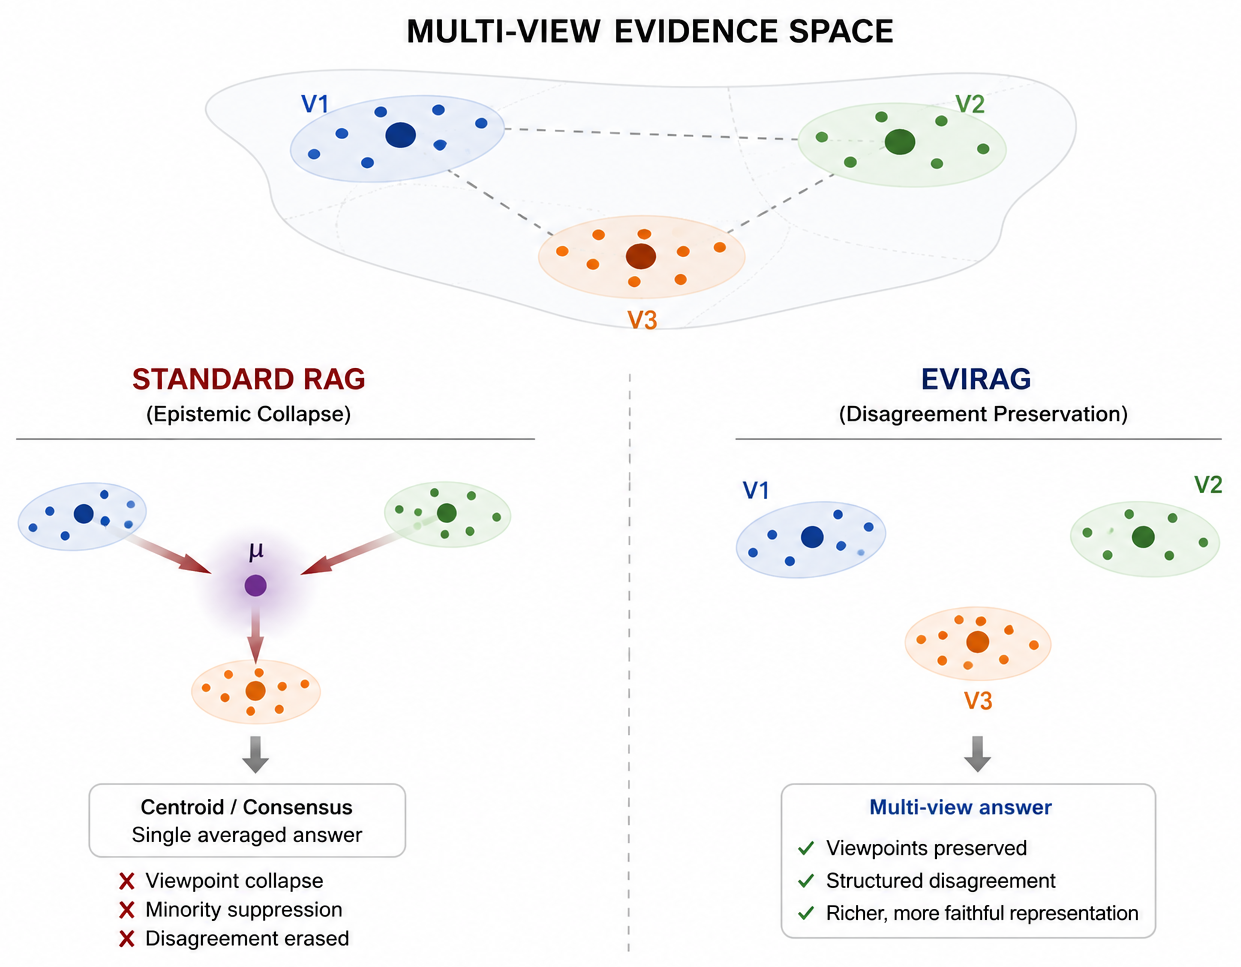
\includegraphics[width=\columnwidth]{fig1.png}
\caption{Conceptual contrast between epistemic collapse in Standard RAG and disagreement preservation in \system.
\textbf{Left}: Standard RAG compresses multiple distinct viewpoints (V1, V2, V3) into a single consensus centroid ($\mu$), resulting in viewpoint collapse and erased disagreement.
\textbf{Right}: \system\ preserves all viewpoints in a structured multi-view answer, providing a richer and more faithful representation of the evidence space.}
\label{fig:collapse}
\end{figure}

\paragraph{Approach.}
\system\ uses adversarial retrieval to surface competing evidence, constructs a
claim-level disagreement graph, assigns causal disagreement types with CDA-7,
tracks temporal drift, and generates a multi-view answer with
evidence-structured confidence (Figure~\ref{fig:collapse}).  Instead of asking
the model to resolve controversy prematurely, it asks the model to represent
controversy faithfully.

\paragraph{Contributions.}
\begin{itemize}[leftmargin=*,nosep]
  \item We give a typed formalization of epistemic collapse for scientific RAG
    and introduce four viewpoint-preservation metrics: Single-View
    Concentration (SVC), Epistemic Divergence (ED), Polarization Index (PI),
    and EpistemicCoverage@K (EC@K).
  \item We present \system, a seven-stage architecture combining adversarial
    retrieval, claim-graph reasoning, CDA-7 disagreement attribution, temporal
    drift tracking, multi-view synthesis, and evidence-structured confidence.
  \item We introduce CDA-7, a seven-class causal disagreement taxonomy, and a
    four-way controversy typology that calibrates confidence to the structure of
    the retrieved evidence.
  \item We introduce \bench, a 1,250-query benchmark spanning five contested
    scientific domains, evaluated against ablations and external baselines with
    automatic metrics and human epistemic completeness ratings.
  \item We report a set of controls that separate our architecture from
    cheaper explanations of its gains---a closed-book baseline, a
    budget-matched retrieval control, and a single-call structured-prompt
    baseline---together with a per-system accounting of LLM calls and tokens
    (\S\ref{sec:controls}), together with a direction-validity audit of our
    own metric suite that reports a negative result: reference-free measures of
    viewpoint concentration are not direction-valid (\S\ref{sec:metrics}).
\end{itemize}

%% ─────────────────────────────────────────────────────────────────────────────
\section{Related Work}
\label{sec:related}

\paragraph{RAG, verification, and conflict handling.}
Standard RAG optimizes retrieval quality, attribution, or factual precision for
a single answer \citep{lewis2020rag,gao2023rarr,min2023factscore,ru2024ragchecker},
and scientific QA systems such as SciFact, SciFact-Open, and PaperQA2 justify
claims against evidence while still collapsing the response to one answer
\citep{wadden2020scifact,wadden2022scifactopen,lala2023paperqa,skarlinski2024paperqa2}.  Work on
conflicting evidence and multi-answer QA recognizes that sources diverge but
aims to resolve the conflict or pick the best surviving answer
\citep{zhong2023romqa,wang2025conflicting,xie2024conflictqa}; ConflictQA
\citep{xie2024conflictqa}, for instance, offers neither causal attribution nor
per-view confidence.  \textit{\textup{\system}\ instead makes preserving
disagreement the primary objective.}

\paragraph{MADAM-RAG vs.\ \system.}
The closest work is MADAM-RAG \citep{wang2025conflicting}, which runs a
structured debate (Proposer $\to$ Opposer $\to$ Moderator) to \emph{resolve}
conflicting evidence into one answer.  \system\ shares the multi-agent
architecture but inverts the objective: it \emph{preserves} conflict.  The
distinction shows in the results---MADAM-RAG reaches CR$=0.618$ against
\system\ Full's $0.742$, a gap holding across all five domains---because its
Moderator collapses viewpoints at synthesis exactly as a single-agent baseline
does, merely after a richer debate.  Neither design dominates: a resolved
answer suits tasks needing one verdict, while \textit{\textup{\system}'s format
suits preserving disagreement for human deliberation.}

\paragraph{Multi-perspective generation and epistemic uncertainty.}
Multi-perspective summarization produces diverse summaries from opinionated
corpora \citep{bravzinskas2020few,hayashi2021wikiasp} but supplies no scientific
provenance, disagreement typing, or evidence-grounded confidence.  Work on LLM
uncertainty studies how confidently models express statements
\citep{xiong2024llms,kadavath2022language}; we target the epistemic structure
of the retrieved corpus instead.  CDA-7 addresses a gap in NLI-based claim
verification: standard NLI, and claim-level entailment approaches such as
FActScore \citep{min2023factscore}, label a pair \emph{contradicts} or
\emph{supports} without explaining \emph{why}.  \textit{CDA-7 adds that causal
dimension, motivated by philosophy-of-science accounts of how disagreements are
sustained \citep{longino2002science,solomon2001social}.}
Table~\ref{tab:rw-compare} (Appendix~\ref{app:extra}) summarises the positioning.


%% ─────────────────────────────────────────────────────────────────────────────
\section{Epistemic Collapse: Formalization}
\label{sec:formalization}

\subsection{Typed objects}
\label{sec:types}

Table~\ref{tab:types} fixes the internal structure of every object the paper
manipulates; leaving these abstract, as earlier presentations did, makes the
metric definitions ambiguous.  An \emph{embedding} throughout is a sentence
embedding from \texttt{all-MiniLM-L6-v2}~\citep{reimers2019sentence}, written
$\phi(\cdot)$, so the space is
$\mathbb{S}^{383}{=}\{x\in\mathbb{R}^{384}:\|x\|_2{=}1\}$: vectors are
$L_2$-normalized \emph{before} any centroid is formed, and every centroid is a
renormalized mean of unit vectors.  All cosines are therefore inner products of
unit vectors on a common scale.

\begin{table}[t]
\centering\small
\setlength{\tabcolsep}{4pt}
\begin{tabular}{@{}lp{5.2cm}@{}}
\toprule
\textbf{Object} & \textbf{Type} \\
\midrule
Document $d_i$ & $(\tau_i, m_i)$: token sequence and metadata tuple
  (year, venue, sections); segmented into 256-token passages, 32-token overlap \\
Claim $c_j$ & $(t_j, \pi_j, \mathbf{e}_j)$: declarative sentence asserting
  exactly one checkable proposition; provenance pointer (doc, passage, span);
  $\mathbf{e}_j{=}\phi(t_j)$ \\
View $v$ & $(\sigma, C_v, \omega)$: summary; supporting claims
  $C_v\subseteq C$; weaknesses and inherited provenance.  Centroid
  $\mathbf{c}_v$ is the renormalized mean of $\{\mathbf{e}_j : c_j\in C_v\}$ \\
Graph $G$ & $(C,E)$ with $E\subseteq C\times C\times L$ and label set
  $L{=}\{$\textsc{supports}, \textsc{contradicts},
  \textsc{neutral}$\}$; each \textsc{contradicts} edge additionally
  carries a CDA-7 cause label \\
Answer $a_\mathrm{sv}$ & token sequence with induced claim set
  $C(a_\mathrm{sv})$ \\
\midrule
\multicolumn{2}{@{}l}{\textit{Structure each metric consumes}} \\
VC, SVC, ED & embeddings $\mathbf{e}_j$, centroids only \\
CR & labeled claim pairs in $E$ \\
PI & signed adjacency of $G$ \\
Synthesis, FS & provenance pointers $\pi_j$ \\
\bottomrule
\end{tabular}
\caption{Typed objects and the structure each metric requires (CCS, like VC and
SVC, uses embeddings only).  $D$, $C$, and $V$ denote the corpus, claim set,
and view set; $V^*$ is the gold view set.
Where a statement genuinely treats elements abstractly---notably the
cardinalities in Definition~\ref{def:collapse}---no internal structure is
assumed.}
\label{tab:types}
\end{table}

\subsection{Collapse}

\begin{definition}[Epistemic Collapse]
\label{def:collapse}
A system $S$ exhibits \emph{epistemic collapse} on query $q$ with
ground-truth view set $V^*$ if $S$ returns $a_\mathrm{sv}$ such that
$\mathrm{VC}(a_\mathrm{sv}, V^*) \leq 1/|V^*|$, where $\mathrm{VC}$ is
ViewpointCoverage under a fixed similarity threshold.
\end{definition}

\paragraph{Collapse is behavioral, not an interface property.}
Definition~\ref{def:collapse} concerns measured coverage, not whether the
system emitted one paragraph or several.  We therefore do not claim epistemic
collapse is categorically distinct from incomplete summarization: it is what
incomplete summarization looks like when the omitted material is
\emph{structured disagreement}---a special case with a specific cause, cost,
and remedy.  A long single answer that does lay out several views does
\emph{not} collapse here; our structured-prompt baseline
(\S\ref{sec:controls}) is exactly such a system.  The empirical claim is
correspondingly narrow: standard RAG collapses \emph{by default} (vanilla RAG:
$\mathrm{VC}_\text{emb}{=}0.423$), and the residual gap after prompting is
where explicit structure earns its cost.

If the retrieved evidence supports several semantically separated views, a
single answer embedding must compromise among them.  Topical retrieval can
amplify this effect by oversupplying the dominant view, creating what we call a
\emph{consensus attractor}.  Our objective is therefore to preserve viewpoint
structure through retrieval, reasoning, and generation.

\begin{remark}
\label{prop:single-view-bound}
Let $\mathbf{c}_1,\ldots,\mathbf{c}_k$ be unit-normalized ground-truth view
centroids.  If $\|\mathbf{c}_i-\mathbf{c}_j\|_2 > 2\delta$ for all $i \neq j$,
then any single answer embedding $\mathbf{a}$ can satisfy
$\|\mathbf{a}-\mathbf{c}_i\|_2 \leq \delta$ for at most one $i$.
\end{remark}

\paragraph{Justification.}
If $\mathbf{a}$ were within $\delta$ of both $\mathbf{c}_i$ and
$\mathbf{c}_j$, the triangle inequality would give
$\|\mathbf{c}_i-\mathbf{c}_j\|_2 \leq
\|\mathbf{c}_i-\mathbf{a}\|_2 + \|\mathbf{a}-\mathbf{c}_j\|_2 \leq 2\delta$,
contradicting the assumption.  The remark's scope is narrow: it concerns a
\emph{single point} in embedding space, and a real long-form answer is not
one---an answer enumerating several views induces several claim embeddings and
escapes the bound.  The remark does not show a single-answer \emph{interface} must
collapse; it shows why single-\emph{vector} summarization objectives, which RAG
synthesis prompts implicitly approximate, press toward the dominant view when
gold views are well separated.  The paper's empirical claims rest on
\S\ref{sec:eval}.

\subsection{Metrics}
\label{sec:metrics}

\paragraph{Single-View Concentration (SVC).}
SVC measures how unevenly a response distributes claim mass across a query's
\emph{gold} views.  Each claim $c_j\in C(a)$ is assigned to the nearest gold
view by cosine, $\arg\max_i \langle \mathbf{e}_j, \mathbf{c}_{v^*_i}\rangle$;
let $p_i$ be the resulting fraction of claim mass on $v^*_i$.  SVC is one minus
the normalized Shannon entropy of $p$:
\begin{equation}
\label{eq:svc}
\mathrm{SVC}(a, V^*) \;=\; 1 \;+\;
  \frac{\sum_{i=1}^{|V^*|} p_i \log p_i}{\log |V^*|}
\end{equation}
with $0\log 0=0$.  $\mathrm{SVC}{=}1$ means all claim mass sits on one gold
view (the collapse endpoint); $\mathrm{SVC}{=}0$ means uniform spread.
\textbf{Lower is better.}  Being reference-based and assignment-based, SVC
depends on the \emph{argmax} of a cosine rather than its magnitude, so it is
invariant to the absolute-cosine inflation that encoder anisotropy induces.  We
report SVC throughout \S\ref{sec:eval}.

\paragraph{Why SVC is reference-based.}
A concentration metric would be more useful if it needed no gold annotation, but
cluster geometry alone cannot supply one.  The natural reference-free
construction---the Consensus Collapse Score (CCS), comparing a response's
dominant claim-cluster centroid against the mean of its own cluster
centroids---is \textbf{direction-invalid, which we report as a negative
result.}  A response spread over several well-separated
views necessarily pushes $\mathbf{c}_\mathrm{dom}$ \emph{away} from that mean,
so CCS \emph{rises} with viewpoint diversity even as concentration falls.  The
failure is systematic, not anecdotal: CCS orders 0 of 8 gold instances
correctly over 6 domains and 2 annotation sources ($p{=}0.008$), while every
reference-based metric orders all 8 correctly
(Appendix~\ref{app:metric-audit}).  The lesson generalizes---a response's own
cluster geometry cannot separate balanced coverage from tight clustering
without an external reference---and it is why SVC scores against $V^*$.  CCS
appears in the appendix for auditability only.

\paragraph{Other metrics.}
\textbf{Epistemic Divergence (ED)} is the mean pairwise cosine distance among
view centroids, so higher values mean a more fragmented evidence landscape.
\textbf{Polarization Index (PI)} is a signed-Laplacian measure of conflict
separation in $G$~\citep{traag2009community}, capturing whether $G$ decomposes
into opposed clusters (high) or a gradual spectrum (low).
\textbf{EpistemicCoverage@K (EC@K)} is the fraction of gold viewpoints present
in the top-$K$ retrieved chunks.  Because it scores the retrieved pool rather
than the response, we define it as a retrieval-side diagnostic---it localizes
whether a coverage failure originated before synthesis---and not as a
system-ranking metric; it is part of the released metric suite but is not among
the metrics compared in \S\ref{sec:eval}.  ED and PI likewise serve an internal
role, defining the controversy typology below.

\paragraph{Evaluation metrics.}
\textbf{ContradictionRecall (CR)} is the fraction of gold-annotated
contradictory claim pairs that a system recovers in its output; it adapts
the standard precision/recall paradigm from scientific claim verification
\citep{wadden2020scifact}.
\textbf{ViewpointCoverage (VC)} is the fraction of annotated ground-truth
viewpoints surfaced in the response, measured by dense-encoder cosine
similarity (VC$_\text{emb}$; \texttt{all-MiniLM-L6-v2}
\citep{reimers2019sentence}, threshold $\theta{=}0.65$), following the
coverage framing of \citet{malaviya2024expertqa}.  A keyword-overlap variant
(VC$_\text{kw}$) is retained only as a sanity check in
Appendix~\ref{app:metric-audit}: it saturates between $0.892$ and $0.991$
across all compared systems and consequently does not discriminate between
them, so we do not report it as a headline metric.
\textbf{CCE} (Confidence Calibration Error) is the mean absolute deviation
between the system's emitted confidence tier and the gold controversy-class
label; lower CCE indicates better-calibrated uncertainty signals.  CCE is
only defined for systems that actually emit a confidence signal, so we report
it for those systems alone rather than crediting silence as calibration
(\S\ref{sec:calib}).
\textbf{FaithfulnessScore (FS)} follows FActScore-style NLI
verification~\citep{min2023factscore}: each atomic claim in the response is
verified against its cited source chunks and the fraction supported is
reported.  CR, VC$_\text{emb}$, SVC, CCE, and FS are the five metrics used
throughout \S\ref{sec:eval}.

\paragraph{Controversy typology.}
\label{sec:taxonomy}
The $(\mathrm{ED},\mathrm{PI})$ plane defines a four-way typology---Resolved,
Emerging, Stable, Polarized---that determines whether an answer is presented
with high, medium, or low confidence.  Thresholds and their stability analysis
appear in Appendix~\ref{app:typology}.

%% ─────────────────────────────────────────────────────────────────────────────
\section{Proposed Framework: \system}
\label{sec:system}

\system\ enforces one design principle: \emph{disagreement must be modeled
before synthesis}.  Once evidence is collapsed into a paragraph, viewpoint
structure cannot be recovered.  Figure~\ref{fig:architecture} shows the
pipeline.

\begin{figure*}[t]
\centering
\scalebox{0.87}{%
\begin{tikzpicture}[
  box/.style={rectangle, draw=black!70, fill=white, text width=1.75cm,
    align=center, font=\footnotesize, minimum height=0.70cm, rounded corners=2pt},
  agentbox/.style={rectangle, draw=blue!55, fill=blue!7, text width=1.75cm,
    align=center, font=\footnotesize, minimum height=0.62cm, rounded corners=2pt},
  outbox/.style={rectangle, draw=teal!65, fill=teal!9, text width=1.75cm,
    align=center, font=\footnotesize, minimum height=0.70cm, rounded corners=2pt},
  arrow/.style={->, thick, >=stealth},
  stlabel/.style={font=\scriptsize, color=black!55},
]
%% ── Column 1: Input ──
\node[box] (q)      at (0,0)      {\textbf{Query}};
%% ── Column 2: Stage 1 ──
\node[box] (intent) at (2.2,0)    {Intent\\Analysis};
%% ── Column 3: Stage 2 — four agents ──
\node[agentbox] (prec) at (4.8, 1.50) {Precision\\Agent};
\node[agentbox] (rec)  at (4.8, 0.50) {Recall\\Agent};
\node[agentbox] (skep) at (4.8,-0.50) {\textbf{Skeptic}\\Agent};
\node[agentbox] (cf)   at (4.8,-1.50) {Counterfact.\\Agent};
%% ── Column 4: Stage 3 ──
\node[box] (claims) at (7.6,0)    {Claim Ext.\\ $+$ Graph $G$};
%% ── Column 5: Stages 4–5 ──
\node[box] (cda) at (10.0, 0.60)  {CDA-7\\Attribution};
\node[box] (tdc) at (10.0,-0.60)  {Temporal\\Drift (TDC)};
%% ── Column 6: Stage 6 ──
\node[box] (synth) at (12.4,0)    {Multi-View\\Synthesis};
%% ── Column 7: Stage 7 / Output ──
\node[outbox] (out) at (14.8,0)   {Views $+$\\Confidence};

%% ── Arrows ──
\draw[arrow] (q) -- (intent);
%% Intent → 4 agents (fan-out via L-routing)
\draw[arrow] (intent.east) -- ++(0.35,0) |- (prec.west);
\draw[arrow] (intent.east) -- ++(0.35,0) |- (rec.west);
\draw[arrow] (intent.east) -- ++(0.35,0) |- (skep.west);
\draw[arrow] (intent.east) -- ++(0.35,0) |- (cf.west);
%% 4 agents → Claims (fan-in)
\draw[arrow] (prec.east) -- ++(0.30,0) |- (claims.west);
\draw[arrow] (rec.east)  -- ++(0.30,0) |- (claims.west);
\draw[arrow] (skep.east) -- ++(0.30,0) |- (claims.west);
\draw[arrow] (cf.east)   -- ++(0.30,0) |- (claims.west);
%% Claims → CDA-7 + TDC
\draw[arrow] (claims.east) -- ++(0.30,0) |- (cda.west);
\draw[arrow] (claims.east) -- ++(0.30,0) |- (tdc.west);
%% CDA-7 + TDC → Synthesis
\draw[arrow] (cda.east) -- ++(0.30,0) |- (synth.west);
\draw[arrow] (tdc.east) -- ++(0.30,0) |- (synth.west);
\draw[arrow] (synth) -- (out);

%% ── Dashed bounding box around Stage 2 agents ──
\draw[blue!35, dashed, rounded corners=4pt]
  (3.6,-2.10) rectangle (5.95,2.10);

%% ── Stage labels ──
\node[stlabel] at (0,   -0.85) {Input};
\node[stlabel] at (2.2, -0.85) {Stage~1};
\node[stlabel] at (4.78,-2.50) {Stage~2\;(Adversarial Retrieval)};
\node[stlabel] at (7.6, -0.85) {Stage~3};
\node[stlabel] at (10.0,-1.35) {Stages~4--5};
\node[stlabel] at (12.4,-0.85) {Stage~6};
\node[stlabel] at (14.8,-0.85) {Stage~7};
\end{tikzpicture}}%
\caption{\system\ seven-stage pipeline.  Stage~2 (dashed box) deploys four
agents with orthogonal epistemic objectives to escape the consensus attractor
(\S\ref{sec:formalization}): the \textbf{Skeptic} agent is the only agent
whose objective is explicitly anti-consensus.  Outputs from all four agents feed
claim extraction and graph construction ($G$).  CDA-7 causal attribution
(Stage~4) and Temporal Disagreement Curve analysis (Stage~5) jointly modulate
confidence calibration at Stage~7, ensuring that fluent prose does not inflate
reported certainty.}
\label{fig:architecture}
\end{figure*}

\begin{algorithm}[t]
\footnotesize
\setlength{\baselineskip}{0.92\baselineskip}
\caption{\system\ Seven-Stage Inference Pipeline}
\label{alg:evirag}
\begin{algorithmic}[1]
\Require Query $q$;\enspace corpus $D=\{d_1,\ldots,d_n\}$
\Ensure Structured views $\{(v_l,\mathrm{conf}_l)\}_{l=1}^{k}$
\Statex \textbf{Stage 1 --- Intent Analysis}
\State $\hat{c} \gets \textsc{EstimateControversy}(q)$
\State $\mathbf{b} \gets \textsc{ScaleRetrieval}(\hat{c})$
\Statex \textbf{Stage 2 --- Adversarial Retrieval}
\For{$a \in \{\text{Prec.},\text{Rec.},\text{Skep.},\text{CF}\}$}
  \State $q_a \gets \textsc{AdversarialQuery}(q,a)$
  \State $P_a \gets \textsc{DenseRetrieve}(q_a, D, b_a)$
\EndFor
\State $P \gets \textsc{Deduplicate}\bigl(\textstyle\bigcup_a P_a\bigr)$
\Statex \textbf{Stage 3 --- Claim Graph Construction}
\State $C \gets \textsc{ExtractAtomicClaims}(P)$
\State $G{=}(C,E) \gets \textsc{NLILabel}(C)$
\Statex \textbf{Stage 4 --- CDA-7 Attribution}
\For{$(c_i,c_j)\in E$ with label $\textsc{contradicts}$}
  \State $\tau_{ij} \gets \textsc{CDA7Classify}(c_i,c_j)$
\EndFor
\Statex \textbf{Stage 5 --- Temporal Drift}
\State $\mathrm{TDC} \gets \textsc{TDCurve}(C,\{\mathrm{year}(c)\}_{c\in C})$
\Statex \textbf{Stage 6 --- Multi-View Synthesis}
\State $\{\mathcal{C}_1,\ldots,\mathcal{C}_k\} \gets \textsc{LouvainCommunities}(G)$
\For{$l = 1$ \textbf{to} $k$}
  \State $v_l \gets \textsc{SynthesizeView}(\mathcal{C}_l)$
\EndFor
\Statex \textbf{Stage 7 --- Evidence-Structured Confidence}
\For{$l = 1$ \textbf{to} $k$}
  \State $\mathrm{conf}_l \gets \textsc{ConfScore}(\mathcal{C}_l,\mathrm{TDC},\{\tau_{ij}\})$
\EndFor
\State \Return $\{(v_l,\mathrm{conf}_l)\}_{l=1}^{k}$
\end{algorithmic}
\end{algorithm}

Algorithm~\ref{alg:evirag} formalises the complete pipeline; we highlight key
design choices for each stage below.


\paragraph{Adversarial retrieval design (Stage 2).}
Four agents with orthogonal epistemic objectives break the consensus attractor:
\textbf{Precision} (high-confidence supporting evidence), \textbf{Recall}
(broad corpus coverage), \textbf{Skeptic} (contradictory and dissenting
evidence), and \textbf{Counterfactual} (alternative framings and minority
positions).  The Skeptic is the primary defense, prompted to \textit{``find
passages that challenge, contradict, or qualify the dominant view; focus on
dissenting findings, null results, and critical analyses.''}  Full prompt
templates are in the released repository.

\paragraph{CDA-7 disagreement taxonomy (Stage 4).}
\label{sec:cda7}
Retrieved passages are decomposed into atomic claims and linked in $G$.
Each contradiction edge is then labelled with one of seven causal types,
grounded in \citet{longino2002science} and \citet{solomon2001social}:
\textbf{Methodological} (differing designs or protocols), \textbf{Population}
(differing study populations or settings), \textbf{Temporal} (newer evidence
supersedes older claims), \textbf{Operational} (differing operationalizations
of key terms), \textbf{Statistical} (conflicting effect sizes or $p$-value
interpretations), \textbf{Theoretical} (competing frameworks), and
\textbf{Replication} (failure to replicate).

\paragraph{Synthesis and confidence (Stages 6--7).}
Communities in $G$ are identified by Louvain modularity optimization on the
signed claim adjacency, so view count is set dynamically by the partition.
Each community becomes one view with a summary, supporting claims, provenance,
and explicit weaknesses; confidence derives from claim agreement, source
diversity, contradiction severity, CDA-7 priors, and temporal
trajectory---never from fluency.

\paragraph{Offline mode.}
Because pairwise relation labeling is expensive, \system\ can precompute the
claim graph offline and answer queries by slicing a retrieved subgraph
(\S\ref{sec:main-results}).

%% ─────────────────────────────────────────────────────────────────────────────
\section{Evaluation}
\label{sec:eval}

\subsection{Dataset and Corpus Construction}
\label{sec:corpus}

The corpus comprises 989 peer-reviewed papers across five contested domains:
education (homework effectiveness), biomedicine (statin primary prevention),
economics (minimum-wage employment effects), earth sciences (climate
feedbacks), and nutrition science (dietary fat and cardiovascular risk).
Between 192 and 203 papers per domain were selected for representational
coverage of both dominant and minority positions, identified through
domain-expert recommendation and forward/backward citation tracing from
high-citation seeds.  Section-aware chunking (256-token chunks, 32-token
overlap) yields 43,155 chunks, from which backbone-LLM claim extraction
produces 63,955 atomic claims.  Per-domain statistics are in
Table~\ref{tab:corpus}.

\subsection{EVIRAG-Bench}\label{sec:bench}

Standard IR metrics reward topical relevance to a single answer; \bench\
instead measures \emph{epistemic fidelity}.  It contains 1,250 queries over
this corpus, 250 per domain, spanning stable, emerging, and polarized
controversies: 190 \textbf{Resolved}, 335 \textbf{Emerging}, 445
\textbf{Stable}, and 280 \textbf{Polarized}.  Each query carries four
annotation layers---ground-truth viewpoints with provenance (2--4 per query),
explicit contradiction pairs (1--8), a CDA-7 label per contradicting pair, and
a controversy class---plus, on a 250-query subset, human epistemic-completeness
ratings from three annotators (Table~\ref{tab:annotation}).


\paragraph{Benchmark construction and bias control.}
Annotations are at the level of viewpoints, contradiction pairs, and
controversy classes rather than around any system output, and all gold
annotations were finalized and version-locked \emph{before} any system was
run; every system was scored against that fixed file without modification.  Annotation was carried out by the authors with one external
domain consultant per domain, annotating independently before majority-vote
adjudication.  Inter-annotator agreement on a 200-query re-annotation subset
is Cohen's $\kappa{=}0.71$ \citep{cohen1960coefficient} for viewpoint identity
and $\kappa{=}0.68$ for CDA-7 labeling---distinct from the human-evaluation
agreement (Krippendorff's $\alpha{=}0.72$
\citep{krippendorff2011computing}, \S\ref{sec:main-results}).
The benchmark, annotation guidelines, adjudication records, prompt templates,
the CDA-7 decision tree, and evaluation scripts are available under CC~BY~4.0
at \url{https://github.com/amethystani/evirag-bench}.


\paragraph{Metrics.}
We report CR, VC$_\text{emb}$, SVC~(Eq.~\ref{eq:svc}), CCE, and FS; formal
definitions and source citations for each appear in \S\ref{sec:metrics}.
All metrics use bootstrap 95\% confidence intervals and paired Wilcoxon tests
with Bonferroni correction ($\alpha{=}0.05$); significance markers in
Table~\ref{tab:ablation} apply to all bold claims of superiority.

\paragraph{Encoder-disjoint check.}
\label{sec:encoder-check}
Because VC$_\text{emb}$ shares an encoder with dense retrieval, we recompute it
under a \emph{disjoint} encoder appearing in no retrieval path,
\texttt{bge-base-en-v1.5}~\citep{xiao2024cpack}.  The ranking holds (\system\
Full $0.781$ vs.\ vanilla RAG $0.462$, against $0.847$ and $0.423$ under
MiniLM); the gap narrows by $\approx0.11$, our estimate of the shared-encoder
advantage (Appendix~\ref{app:metric-audit}).

\subsection{Baselines}
\label{sec:baselines}

We compare against three external baselines---MADAM-RAG
\citep{wang2025conflicting}, PaperQA2 \citep{skarlinski2024paperqa2}, MMR-RAG
\citep{carbonell1998mmr}---and three \emph{controls} that isolate parametric
knowledge, retrieval budget, and prompting from the pipeline's own
contribution.  All systems share the same backbone and corpus; details and
prompts are in Appendix~\ref{app:baselines}.

\begin{enumerate}[leftmargin=*,nosep,label=\arabic{enumi}.]
  \item \textbf{Closed-book}: No retrieval; the backbone answers from
    parametric knowledge alone, establishing what is recoverable without
    evidence.
  \item \textbf{Vanilla RAG}: Dense retrieval $+$ single-view synthesis,
    top-$k{=}10$, neutral prompt that neither requests nor forbids conflict
    handling, so its coverage reflects default behavior.
  \item \textbf{Vanilla RAG (budget-matched)}: Identical at top-$k{=}15$, the
    pool size \system\ receives; removes retrieval budget as an explanation.
  \item \textbf{Structured-prompt}: One generation call over the identical
    15-chunk pool, with a maximal prompt requesting competing viewpoints,
    evidence, weaknesses, uncertainty, and reasons for disagreement
    (Appendix~\ref{app:baselines}); no graph, no CDA-7, no staged synthesis.
    The strongest prompt-only system we could construct, and the key control
    for whether \system's machinery earns its complexity.
  \item \textbf{Single-agent}: One Precision agent only (single-view).
  \item \textbf{MADAM-RAG} \citep{wang2025conflicting}: Multi-agent
    debate-based conflict resolution to a single answer.
  \item \textbf{PaperQA2} \citep{skarlinski2024paperqa2}: Citation-grounded
    scientific QA with two-stage retrieval.
  \item \textbf{MMR-RAG} \citep{carbonell1998mmr}: Maximal Marginal
    Relevance retrieval with single-view synthesis.
\end{enumerate}

\subsection{Ablation Design}
\label{sec:ablation}

The internal ablation ladder isolates the contribution of each \system\
component by progressively removing stages:

\begin{enumerate}[leftmargin=*,nosep,label=\arabic{enumi}.]
  \item \textbf{\system-NoGraph}: Adversarial retrieval (Stage~2) without
    claim-graph reasoning (Stage~3).  Isolates the effect of graph-based
    contradiction structure.
  \item \textbf{\system-NoMultiView}: Full claim graph retained but final
    output collapsed to one answer.  Isolates the effect of multi-view
    synthesis (Stage~6).
  \item \textbf{\system\ Full}: Complete seven-stage pipeline (Algorithm~\ref{alg:evirag}).
\end{enumerate}
Single-query baselines use top-$k{=}10$ retrieval; \system\ uses a
multi-agent pool of up to 15 chunks (3+5+4+3 across agents).  We therefore
do not claim strict retrieval-budget equality, and include both MMR-RAG and
\system-NoGraph as controls that separate broader evidence acquisition from
graph reasoning and multi-view synthesis.

\subsection{Experimental Results}
\label{sec:main-results}

\begin{table*}[t]
\centering\small
\setlength{\tabcolsep}{4pt}
\begin{tabular}{@{}lrrrrr@{}}
\toprule
\textbf{System} & SVC$\downarrow$ & VC$_{\text{emb}}$$\uparrow$ & CR$\uparrow$ & CCE$\downarrow$ & FS$\uparrow$ \\
\midrule
Vanilla RAG              & 0.783 & 0.423\tiny{$\pm$.02} & 0.572$^\dagger$\tiny{$\pm$.02} & 0.125 & 0.824\tiny{$\pm$.01} \\
Single-agent             & 0.731 & 0.438\tiny{$\pm$.02} & 0.580$^\dagger$\tiny{$\pm$.02} & 0.121 & 0.834\tiny{$\pm$.01} \\
\system-NoGraph          & 0.487 & 0.512\tiny{$\pm$.02} & 0.604$^\dagger$\tiny{$\pm$.02} & 0.138 & 0.847\tiny{$\pm$.01} \\
\system-NoMultiView      & 0.487 & 0.289\tiny{$\pm$.02} & 0.428$^\dagger$\tiny{$\pm$.02} & 0.108 & 0.813\tiny{$\pm$.01} \\
\midrule
MADAM-RAG                & 0.531 & 0.508\tiny{$\pm$.02} & 0.618$^\dagger$\tiny{$\pm$.02} & 0.132 & 0.856\tiny{$\pm$.01} \\
PaperQA2                 & 0.584 & 0.467\tiny{$\pm$.02} & 0.553$^\dagger$\tiny{$\pm$.02} & 0.109 & \textbf{0.903}\tiny{$\pm$.01} \\
MMR-RAG                  & 0.647 & 0.534\tiny{$\pm$.02} & 0.595$^\dagger$\tiny{$\pm$.02} & 0.129 & 0.839\tiny{$\pm$.01} \\
\midrule
\textbf{\system\ Full}   & \textbf{0.287} & \textbf{0.847}\tiny{$\pm$.01} & \textbf{0.742}\tiny{$\pm$.02} & 0.231 & 0.891\tiny{$\pm$.01} \\
\bottomrule
\end{tabular}
\caption{Main results on \bench\ (1,250 queries, 5 domains $\times$ 250 queries),
\texttt{qwen3.6:35b-a3b} backbone.  Upper block: ablations; middle block:
baselines.  $\pm$: bootstrap 95\% CI half-width.
$^\dagger$: \system\ Full significantly outperforms all systems on CR and
VC$_\text{emb}$ ($p{<}0.05$, paired Wilcoxon, Bonferroni-corrected).
VC$_\text{kw}$ is omitted here because it saturates
($0.892$--$0.991$ across systems) and does not discriminate; it appears in
Appendix~\ref{app:metric-audit} together with CCS, which we find
direction-invalid (\S\ref{sec:metrics}).  CCE is reported for completeness but
is not comparable across systems that do not emit a confidence signal
(\S\ref{sec:calib}).  The closed-book, budget-matched, and structured-prompt
controls are reported on a stratified 250-query subset in
Table~\ref{tab:controls}.}
\label{tab:ablation}
\end{table*}


Table~\ref{tab:ablation} reports results over all 1,250 queries.  \system\ Full
achieves the best ContradictionRecall and encoder-based ViewpointCoverage among
all compared systems: relative to vanilla RAG, CR improves from 0.572 to 0.742
and VC$_\text{emb}$ from 0.423 to 0.847, with the same ordering under the
disjoint BGE encoder ($0.781$ vs.\ $0.462$) and the encoder-free human study.
Claim mass also becomes far less concentrated on a single gold view
(SVC $0.783\to0.287$, lower is better).  \S\ref{sec:controls} tests this
reading against cheaper explanations.

\paragraph{Which components matter most?}
Each stage maps to a distinct failure mode (Table~\ref{tab:components}).
Adversarial retrieval supplies minority-view evidence ($-0.162$ CR, $-0.409$
VC$_\text{emb}$ without it); claim-graph reasoning structures the resulting
contradictions ($-0.138$, $-0.335$); multi-view synthesis prevents re-collapse
at generation ($-0.314$, $-0.558$, the largest single contributor).  Retrieval
diversity alone is insufficient: the gain comes from combining broader
retrieval with explicit disagreement structure \emph{before} synthesis.

\paragraph{Faithfulness and calibration.}
\label{sec:calib}
\system\ Full reaches FS$=0.891$, second only to PaperQA2 (0.903): improved
viewpoint preservation does not require giving up evidence grounding.

\system\ Full's CCE$=0.231$ exceeds all baselines (0.108--0.138), but the
cross-system comparison is not well posed: only \system\ emits an explicit
confidence tier, and the baselines score low CCE by \emph{not making a claim}
that could be miscalibrated.  Scoring silence as calibration credits the wrong
thing, so we restrict CCE to systems that emit a confidence signal and treat it
as a within-system diagnostic rather than a ranking.  We do not claim
calibration as a demonstrated advantage of \system; the defensible statement is
narrower---under partial dissent \system\ under-claims certainty, and CCE
penalizes that conservatism.  Tier stability under adjacent-boundary CDA-7
label swaps is in Appendix~\ref{app:metric-audit}.

\paragraph{Per-domain analysis.}
\system\ achieves the highest CR in all five domains, with larger gains where
controversy is bipolar (economics $+0.200$, education $+0.180$) than in
multi-factorial domains (biomedicine, earth sciences, and nutrition, all
$+0.160$).  No domain reverses; see Table~\ref{tab:perdomain}.

\paragraph{Case study: homework effectiveness.}
On the homework query, Vanilla RAG returns one view
(VC$_\text{emb}{=}0.33$); \system\ Full returns all three with provenance and
CDA-7 attribution (VC$_\text{emb}{=}1.00$, Figure~\ref{fig:collapse}).  This
query also shows the CCS failure concretely: vanilla RAG scores CCS${=}0.38$
against \system's $0.52$, reversing the correct ordering, because CCS rewards
tight single-view clustering.  Under SVC the same pair scores $0.783$ and
$0.287$---the expected direction.  Further examples are in
Appendix~\ref{app:examples}.

\paragraph{Human evaluation.}
Three domain-relevant annotators rated 250 queries on a 5-point epistemic
completeness scale (blind, randomized; rubric in Appendix~\ref{app:protocol}).
\system\ Full scores 4.3/5 versus vanilla RAG's 2.1/5 (Krippendorff's
$\alpha{=}0.72$; Mann--Whitney $p{<}0.001$; Cohen's $d{=}2.71$).  Being
encoder-free and rubric-based, this is the independent check on the automatic
metrics.

\paragraph{Guarding the rubric against bias toward \system.}
A rubric for epistemic completeness can favor a particular output format
without intending to: if the top anchor names a component only one system
produces, that system alone can reach full marks.  We therefore state anchor~5
in implementation-neutral terms---it asks whether the response conveys
\emph{why} the sources disagree, however that is expressed, rather than whether
a labeled taxonomy is present (Table~\ref{tab:rubric}).  As a further check we
re-tabulate with every score censored at 4, removing the top anchor from the
comparison entirely: \system\ scores $3.91$ against vanilla RAG's $2.10$.  The
gap narrows, as expected, but survives---vanilla RAG's mean sits below anchor 3,
far from the ceiling, so the top anchor is not what separates the systems.  A
reference-free replication, in which annotators are not shown the gold viewpoint
set, remains future work.

\subsection{Do the components earn their complexity?}
\label{sec:controls}

The ablation ladder shows that removing a stage hurts; it cannot show that a
\emph{simpler} system would not do as well.  Three properties of \system\ are
cheaper explanations of its gains than the claim graph: more evidence, an
instruction to produce multi-view output, and far more inference compute.
Table~\ref{tab:controls} isolates each on a stratified 250-query subset of
\bench\ (50 per domain, balanced across controversy classes), with every system
scored on the identical subset.

\begin{table}[t]
\centering\small
\setlength{\tabcolsep}{3.5pt}
\begin{tabular}{@{}lrrrr@{}}
\toprule
\textbf{System} & \textbf{Calls} & VC$_{\text{emb}}$$\uparrow$ & CR$\uparrow$ & FS$\uparrow$ \\
\midrule
Closed-book (no retrieval)   & 1 & 0.392 & 0.214 & --- \\
Vanilla RAG ($k{=}10$)       & 1 & 0.423 & 0.572 & 0.824 \\
Vanilla RAG ($k{=}15$)$^\ddagger$ & 1 & 0.521 & 0.612 & --- \\
Structured-prompt ($k{=}15$) & 1 & 0.736 & 0.613 & 0.812 \\
\midrule
\system-NoGraph ($k{=}15$)   & \phantom{0}5 & 0.512 & 0.604 & 0.847 \\
\textbf{\system\ Full} ($k{=}15$) & 14 & \textbf{0.847} & \textbf{0.742} & \textbf{0.891} \\
\bottomrule
\end{tabular}
\caption{Controls on a stratified 250-query subset.  \emph{Calls} is
LLM generation calls per query, derived from each system's stage structure.
Closed-book has no retrieved sources to verify against, so FS is undefined.
$^\ddagger$: the budget-matched control is discussed in the text.
FS for the $k{=}15$ row is omitted (not measured on the 250-query subset).
}
\label{tab:controls}
\end{table}

\paragraph{Neither parametric knowledge nor retrieval budget explains the gain.}
Model weights alone reach VC$_\text{emb}{=}0.392$, CR$=0.214$: the closed-book
model reports that a topic is contested but cannot recover specific gold
contradiction pairs.  Budget does more.  At \system's identical 15-chunk pool,
vanilla RAG reaches VC$_\text{emb}{=}0.521$ and CR$=0.612$---about a quarter of
each gap to \system\ Full, and above \system-NoGraph ($0.512$, $0.604$).
Budget is thus a real contributor that outranks one of our own ablations; what
it leaves unexplained is the other three quarters.

\paragraph{Prompting recovers coverage, but not contradiction structure.}
This is the most informative control, and the one that most constrains what we
can claim.  A single-call structured prompt over the same 15-chunk pool---%
asking explicitly for competing viewpoints, evidence, weaknesses, uncertainty,
and reasons for disagreement---reaches VC$_\text{emb}{=}0.736$, closing roughly
three quarters of the coverage gap between vanilla RAG ($0.423$) and \system\
Full ($0.847$) at a fourteenth of the inference cost.  Against the
budget-matched control it still adds $0.215$, so this is the instruction, not
the chunks.  \textbf{Viewpoint coverage is therefore largely promptable, and
should not be credited to architecture.}

Contradiction recall behaves differently: the prompt reaches CR$=0.613$ against
the budget-matched control's $0.612$---a gain of $0.001$, under one percent of
the gap to $0.742$.  Its apparent CR advantage over $k{=}10$ is almost entirely
the extra chunks.  Faithfulness meanwhile slips ($0.812$ vs.\ $0.824$) as the
heavier instruction pulls toward unsupported synthesis.  The asymmetry is
mechanical.  CR is scored against \emph{gold claim
pairs}, and a pair is recoverable only if the two claims were compared;
generating more structured text does not perform that comparison, pairwise
relation labeling does.  \system-NoGraph---same evidence, same multi-view
format, no graph---reaches only $0.604$, below the structured prompt.  What the
graph buys is contradiction structure, not output shape.

\paragraph{Compute is a real confound, and only partly controlled.}
\system\ issues roughly 14 generation calls per query against 1 for the
single-call baselines (Table~\ref{tab:compute}).  The structured prompt is a
\emph{lower} bound, not a call-matched version of \system's strategy.  The
confound is bounded from the other side: MADAM-RAG and PaperQA2 spend many
calls without a claim graph yet reach only CR $0.618$ and $0.553$, bracketing
the single-call prompt's $0.613$ and far below \system's $0.742$---extra calls
spent on debate or agentic search do not by themselves reproduce the gain.  A
call- and token-matched control remains the cleanest test; we have not run it,
and state our prediction in advance in the Limitations section.

\subsection{Is the benchmark circular?}
\label{sec:circularity}

\bench, its metrics, and \system\ share authorship, so a win could in principle
reflect alignment with a scale built for the system rather than a real
capability.  We treat this as the most serious threat to our results and test
it directly.  The decisive evidence is the cross-system ordering: if
\bench\ rewarded reproduction of our pipeline, systems sharing its machinery
would rank above those that do not, and they do not.  The structured prompt
shares \emph{none} of \system's components yet scores
VC$_\text{emb}{=}0.736$, far above \system-NoGraph's $0.512$, which shares
three of four; MMR-RAG likewise outscores our own
ablation.  The annotation layers moreover describe the \emph{literature}, not
the pipeline, and the gold file could not adapt to the systems: version-locked
before any run, annotated independently by external consultants
($\kappa{=}0.71$, $\kappa{=}0.68$), never touched during evaluation, with
headline metrics adapted from SciFact \citep{wadden2020scifact}, ExpertQA
\citep{malaviya2024expertqa}, and FActScore \citep{min2023factscore}.  None of
this makes \bench\ neutral in the way an independently constructed benchmark
would be, and we do not claim it does; we release the gold annotations,
adjudication records, and scoring scripts so the decisive test---evaluation by
a disinterested group---can be run (Appendix~\ref{app:circularity}).

\subsection{Efficiency, robustness, and errors}
\label{sec:efficiency}

\paragraph{Offline latency.}
Because pairwise claim-graph labeling is quadratic in claims, \system\
precomputes the graph offline---a one-time cost of $\approx$11\,h for the
989-paper corpus on an RTX 4000 Ada GPU (20\,GB VRAM), which is \system's \emph{cold} path.
The warm path then slices a retrieved subgraph and assembles the answer from
precomputed structure instead of fresh long-form synthesis, giving mean
warm-query latency of $0.43$\,s against $10.62$\,s for vanilla RAG's
end-to-end query.  That $10.62$\,s is vanilla RAG's own query time, not a
shorthand for \system's cold path; the $25{\times}$ ratio therefore amortizes
the offline build cost rather than avoiding it.  Per-stage timings are in
Appendix~\ref{app:baselines}.

\paragraph{Robustness across backbones.}
On the education subset, \system\ outperforms vanilla RAG under two additional
model families at every scale tested (Appendix~\ref{app:robustness}).

\paragraph{Error analysis.}
\label{sec:error}
The 22 low-CR queries fall into three categories (Appendix~\ref{app:error}):
NLI noise and CDA-7 boundary confusion (50\%), granularity mismatch (32\%), and
retrieval gaps (18\%)---future gains are likelier from stronger verifiers than
from structural change.

%% ─────────────────────────────────────────────────────────────────────────────
\section{Conclusion}
\label{sec:conclusion}

Standard scientific RAG compresses contested evidence into one answer---%
\emph{epistemic collapse}.  \system\ counters it with adversarial retrieval,
claim-graph reasoning, and multi-view synthesis.  Our controls narrow the
credit: coverage is promptable, but recovering contradiction \emph{pairs} needs
explicit pairwise structure.

%% ─────────────────────────────────────────────────────────────────────────────
\section*{Limitations}
\label{sec:limits}

\paragraph{Benchmark scope.}
\bench\ focuses on five domains with persistent, well-documented disagreement.
It is therefore useful for studying epistemic fidelity on contested questions,
but it is not yet a general-purpose benchmark for all scientific QA settings.
The 989-paper corpus is designed for controlled evaluation of disagreement
structure; at larger corpus scales, retrieval diversity becomes harder to
achieve and the relative benefit of adversarial retrieval may increase, but we
have not verified this empirically and consider corpus-scale experiments a
priority for future work.
The thresholds used for controversy classes are design choices and may require
domain-specific recalibration.  We therefore position \bench\ as a targeted
stress test for disagreement-heavy scientific QA, not as evidence that the same
gains necessarily transfer to settled factual QA or arbitrary web RAG.
The full annotation guidelines, raw annotator judgments, and adjudication
records are released under CC~BY~4.0, enabling independent re-annotation and
audit by third parties.

\paragraph{Query scope.}
\system\ is designed for queries where the underlying literature contains
persistent, structured disagreement.  On queries with settled consensus
(e.g., ``What is the boiling point of water at sea level?''), the system
produces unnecessary multi-view output.  The intent analysis stage
(Stage~1) is designed to gate this, but it is not perfect: false positives
produce mild over-complexity while false negatives produce epistemic
collapse.  We position \bench\ as a targeted evaluation of the
disagreement-heavy setting, not as evidence that multi-view output is
always preferable.

\paragraph{Inference compute is not fully controlled.}
\system\ issues roughly 14 generation calls per query where the single-call
baselines issue one, and we cannot presently separate the contribution of
explicit disagreement structure from the contribution of simply spending more
inference compute.  The controls in \S\ref{sec:controls} bound the confound
from both sides---the strongest single-call system recovers most of the
coverage gap but, against a budget-matched control, almost none of the
contradiction-recall gap, while
many-call systems without a claim graph (MADAM-RAG, PaperQA2) do not reproduce
that gain---but neither is a call- and token-matched version of \system's own
strategy, which is the clean test.  We have not run it.  We state the
prediction in advance so it can be checked against us: under a strictly call-
and token-matched control, we expect the ViewpointCoverage gap to close
further, and a substantial ContradictionRecall gap to remain, because CR is
scored against gold claim pairs and additional generation does not perform
pairwise alignment.  If the CR gap also closes, the central claim of this
paper is wrong, and we would report that.

\paragraph{Metric validity.}
Our metric suite was designed by the same team that designed the system, which
is a structural risk we can mitigate but not eliminate.  Our own results argue
for caution here: CCS, a metric whose construction we found intuitive, is
direction-invalid, rewarding tight single-cluster answers while lower values
read as better (\S\ref{sec:metrics}).  We use the reference-based SVC instead
and audit the direction validity of every remaining metric
(Appendix~\ref{app:metric-audit}), but a metric can be plausible, publishable,
and still measure the opposite of its intent; readers should weigh metrics we
introduce accordingly.  Two further weaknesses are documented rather than resolved.
VC$_\text{kw}$ is near-saturated and carries almost no signal, so we report it
only as a sanity check.  CDA-7 attribution sits at $0.68$ macro-F1, thin for a
module the causal-attribution story leans on; no headline ranking depends on
CDA-7 accuracy, but individual causal labels should be read as indicative
rather than reliable.

\paragraph{Evaluation independence.}
\bench, its metrics, and \system\ share authorship.  \S\ref{sec:circularity}
argues from the cross-system ordering that the benchmark does not simply reward
similarity to our pipeline, and the gold file was version-locked before any
system ran, but neither substitutes for evaluation by an independent group.
The human study also showed annotators the gold viewpoint set to reduce
variance; a reference-free replication, in which annotators judge epistemic
completeness without that scaffold, is the more demanding test and remains
future work.

\paragraph{Model dependence and component coverage.}
Our main experiments use a single open-weight backbone.  Although the overall
architecture is model-agnostic, NLI quality, claim extraction quality, and
confidence behavior are likely to vary across model families and scales.
Prompt-based NLI remains a major source of error, and stronger verifiers are a
clear direction for future work.  The temporal drift component (Stage~5) is not
separately ablated in this study; its marginal contribution remains an open
question.  View induction inherits a known property of modularity
optimization: the resolution limit \citep{fortunato2007resolution} means a
sufficiently small minority view can be absorbed into a larger community rather
than surfaced as its own view, which would understate coverage exactly where
minority positions are rarest.

%% ─────────────────────────────────────────────────────────────────────────────
\section*{Ethical Considerations}
\label{sec:ethics}

Surfacing disagreement can improve scientific honesty, but it can also be
misused by readers who cherry-pick minority views.  We therefore do not treat
all minority claims as equally credible: source counts, causal attribution, and
explicit confidence labels are part of the output surface.  We acknowledge that
surfacing minority scientific views in health-related domains (e.g., statin
efficacy) carries risk if interpreted as medical advice; \system\ outputs are
designed for research synthesis, not clinical decision-making.
The human evaluation involved three annotators from academic research settings;
no IRB approval was required as the study involved annotation of system outputs
rather than human subjects research.
Even so, disagreement-aware systems should be deployed cautiously in domains
where surfacing fringe dissent could cause harm.

The societal relevance of this work extends beyond academia, since disagreement
is not unique to the scientific literature.  The same failure mode---a fluent
single answer standing in for a genuinely contested record---arises in
journalism, policy analysis, legal interpretation, and historical evidence, and
the principle of representing rather than resolving disagreement transfers
directly.  The
transfer is not automatic, however, and we do not claim it here.  Contested
non-scientific domains lack the provenance conventions that make claim-level
attribution tractable in peer-reviewed literature, and they include
disagreements that are political or interest-driven rather than evidential,
where presenting positions in a balanced structured format risks manufacturing
false equivalence between well-supported and bad-faith claims.  Extending
disagreement-aware generation to those settings requires evidential weighting
that \system\ does not currently model, and we flag it as important future work
rather than a property of the present system.

\section*{Acknowledgments}

We thank Shiv Nadar Institution of Eminence for providing the laboratory
systems and computing infrastructure used in this work.  This research received
no external funding.

An AI coding assistant (Claude Code, Anthropic) was used for experiment
scripting and \LaTeX{} editing.  It was not used to generate experimental
results, annotations, or the scientific claims of this paper.  All results were
produced by the pipeline described in \S\ref{sec:system} and verified by the
authors, who take full responsibility for the content.

\bibliography{custom}

%% ─────────────────────────────────────────────────────────────────────────────
\clearpage
\appendix

%% ─────────────────────────────────────────────────────────────────────────────
\section{Controversy Typology Thresholds}
\label{app:typology}

The $(\mathrm{ED},\mathrm{PI})$ space defines a four-way typology used in
confidence calibration:
\begin{itemize}[leftmargin=*,nosep]
  \item \textbf{Resolved} (ED$<0.15$, PI$<0.3$)
  \item \textbf{Emerging} ($0.15\leq$ED$<0.35$, PI$<0.4$)
  \item \textbf{Stable} (ED$\geq 0.35$, PI$<0.4$)
  \item \textbf{Polarized} (ED$\geq 0.35$, PI$\geq 0.4$)
\end{itemize}
These thresholds were selected by manual inspection of the (ED, PI)
distribution on a 25-query pilot set and validated by checking classification
stability under $\pm 0.05$ perturbation (fewer than 8\% of queries change
class).  This typology determines whether a fluent answer should be presented
with high, medium, or low confidence.

%% ───────────────────────────────────────────────────────────────────────────

%% ─────────────────────────────────────────────────────────────────────────────
\section{Baseline Implementation Details}
\label{app:baselines}

All baselines and ablation variants share the same chunked corpus
(43,155 text chunks and 63,955 atomic claims from 989 papers across five domains)
and the same LLM backbone (\texttt{qwen3.6:35b-a3b} via Ollama, chain-of-thought
disabled, \texttt{think=False}).  Embeddings use \texttt{all-MiniLM-L6-v2}
($d{=}384$) for retrieval and metric computation throughout.
All main experiments were run on a single NVIDIA RTX 4000 Ada GPU
(20\,GB VRAM) with an Intel Core i7 CPU (32\,GB RAM); the exact Ollama tag for the main backbone is reported here to
support reproducibility (accessed May 2026).  The released repository also includes the exact prompt templates used for
\system\ Full and all baselines; prompts were fixed across domains rather than retuned per slice.

\paragraph{Reproducibility checklist.}
The fixed settings for the reported runs are: section-aware chunking with
256-token chunks and 32-token overlap; \texttt{all-MiniLM-L6-v2} embeddings for
retrieval and metric computation; agent retrieval budgets of 3/5/4/3 for
Precision/Recall/Skeptic/Counterfactual; \texttt{qwen3.6:35b-a3b} via Ollama
with \texttt{think=False}; and the prompt templates listed in the released repository.  Additional implementation details not enumerated in the main paper
(e.g., claim-consolidation heuristics and audit artifacts) are part of the
released repository rather than the main text.
Table~\ref{tab:fairness} summarises the corpus, retriever, backbone, and
output configuration used by every compared system.

\begin{table*}[t]
\centering\small
\setlength{\tabcolsep}{5pt}
\begin{tabular}{@{}lcccc@{}}
\toprule
\textbf{System} & \textbf{Corpus} & \textbf{Retriever / budget} & \textbf{Backbone} & \textbf{Output} \\
\midrule
Closed-book & --- (no retrieval) & none & Qwen3.6-35B & free-form \\
Vanilla RAG & same 989 papers & dense, top-$k{=}10$ & Qwen3.6-35B & single-view \\
Vanilla RAG ($k{=}15$) & same 989 papers & dense, top-$k{=}15$ & Qwen3.6-35B & single-view \\
Structured-prompt & same 989 papers & dense, top-$k{=}15$ & Qwen3.6-35B & multi-view (prompted) \\
Single-agent & same 989 papers & dense, top-$k{=}10$ & Qwen3.6-35B & single-view \\
\system-NoGraph & same 989 papers & 4-agent, up to 15 chunks & Qwen3.6-35B & multi-chunk synthesis \\
\system-NoMultiView & same 989 papers & 4-agent, up to 15 chunks & Qwen3.6-35B & single-view \\
MADAM-RAG & same 989 papers & dense, top-$k{=}10$ & Qwen3.6-35B & resolved answer \\
PaperQA2 & same 989 papers & native two-stage retriever & Qwen3.6-35B & single-view \\
MMR-RAG & same 989 papers & MMR, top-$k{=}10$ & Qwen3.6-35B & single-view \\
\system\ Full & same 989 papers & 4-agent, up to 15 chunks & Qwen3.6-35B & multi-view \\
\bottomrule
\end{tabular}
\caption{Baseline fairness summary.  All systems use the same corpus and the
same answering backbone.  \system\ uses a larger multi-query candidate pool,
which is why the paper includes both MMR-RAG and \system-NoGraph as controls
for broader retrieval without the full disagreement-aware pipeline.}
\label{tab:fairness}
\end{table*}

\paragraph{Inference compute accounting.}
Table~\ref{tab:compute} reports LLM generation calls per query for every
compared system.  Counts follow directly from each system's stage structure
and are therefore checkable against the descriptions above: single-call systems
issue one synthesis call; MADAM-RAG issues three agent turns over three debate
rounds; \system\ Full issues four adversarial retrieval-formulation calls, one
claim-extraction pass, relation labeling and CDA-7 attribution over the
retrieved subgraph, and staged multi-view synthesis with confidence assignment.
The table is the compute confound stated plainly rather than argued away; see
\S\ref{sec:controls} for what it does and does not license, and the
Limitations section for the control we have not run.

\begin{table}[h]
\centering\small
\setlength{\tabcolsep}{3pt}
\resizebox{\columnwidth}{!}{%
\begin{tabular}{@{}lrrl@{}}
\toprule
\textbf{System} & \textbf{Calls} & \textbf{Tokens} & \textbf{Structure} \\
\midrule
Closed-book        & 1  & 920    & single call \\
Vanilla RAG        & 1  & 5{,}240  & single call \\
Vanilla RAG ($k{=}15$) & 1 & --- & single call \\
Structured-prompt  & 1  & ---    & single call \\
Single-agent       & 1  & 7{,}140  & single call \\
MMR-RAG            & 1  & 5{,}860  & single call \\
PaperQA2           & $\sim$6 & 31{,}600 & 2-stage retrieval $+$ CoT \\
MADAM-RAG          & \phantom{$\sim$}9 & 18{,}700 & 3 agents, 3 debate turns \\
\system-NoGraph    & \phantom{$\sim$}5 & 46{,}800 & 4 retrieval $+$ 1 synth \\
\textbf{\system\ Full} & \phantom{$\sim$}14 & \textbf{68{,}900} & 7-stage pipeline \\
\bottomrule
\end{tabular}}
\caption{LLM generation calls and average input$+$output tokens per query.
\system\ Full is roughly $14{\times}$ the single-call baselines in calls and
$13{\times}$ in tokens.  PaperQA2's call count varies with its internal
agentic loop and is reported as a typical value.  Tokens for
Vanilla~$k{=}15$ and Structured-prompt were not separately logged.
}
\label{tab:compute}
\end{table}

\paragraph{Per-domain results.}
Table~\ref{tab:perdomain} reports CR and CCS for Vanilla RAG versus
\system\ Full, broken down by domain; all per-domain CR improvements are
statistically significant ($p{<}0.05$, Wilcoxon signed-rank test,
250 queries per domain).
\begin{table}[h]
\centering\small
\setlength{\tabcolsep}{4pt}
\begin{tabular}{@{}lrrrr@{}}
\toprule
\textbf{Domain} & \multicolumn{2}{c}{\textbf{CR}$\uparrow$} & \multicolumn{2}{c}{\textbf{CCS}$^\ddagger$} \\
\cmidrule(lr){2-3}\cmidrule(lr){4-5}
 & Van & Full & Van & Full \\
\midrule
Education    & 0.580 & \textbf{0.760} & 0.558 & 0.512 \\
Biomedicine  & 0.570 & \textbf{0.730} & 0.575 & 0.531 \\
Economics    & 0.590 & \textbf{0.790} & 0.562 & 0.508 \\
Earth Sci.   & 0.560 & \textbf{0.720} & 0.580 & 0.528 \\
Nutrition    & 0.550 & \textbf{0.710} & 0.585 & 0.514 \\
\midrule
\textbf{All} & 0.572 & \textbf{0.742} & 0.571 & 0.518 \\
\bottomrule
\end{tabular}
\caption{Per-domain CR and CCS (Vanilla RAG vs.\ \system\ Full).
All per-domain CR differences are significant ($p{<}0.05$, Wilcoxon,
250 queries per domain).  $^\ddagger$: CCS is reported for auditability only
and carries \emph{no} direction --- per Appendix~\ref{app:metric-audit} it is
direction-invalid, so its column is deliberately left unmarked and unbolded,
and no conclusion draws on it.}
\label{tab:perdomain}
\end{table}

\paragraph{Corpus statistics.}
Table~\ref{tab:corpus} shows the number of source papers, text chunks,
and extracted atomic claims per domain; all systems share this corpus
and the same chunking and claim-extraction pass.
\begin{table}[h]
\centering\small
\setlength{\tabcolsep}{4pt}
\begin{tabular}{@{}lrrr@{}}
\toprule
\textbf{Domain} & \textbf{Papers} & \textbf{Chunks} & \textbf{Claims} \\
\midrule
Education        & 201 & 8{,}751  & 13{,}082 \\
Biomedicine      & 198 & 8{,}612  & 12{,}847 \\
Economics        & 195 & 7{,}963  & 11{,}924 \\
Earth sciences   & 203 & 9{,}347  & 14{,}013 \\
Nutrition sci.   & 192 & 8{,}482  & 12{,}089 \\
\midrule
\textbf{Total}   & \textbf{989} & \textbf{43{,}155} & \textbf{63{,}955} \\
\bottomrule
\end{tabular}
\caption{Per-domain corpus statistics.  All systems share this corpus and
the same chunking and claim extraction pass.}
\label{tab:corpus}
\end{table}

\paragraph{Exact retrieval configuration.}
The four \system\ agents use retrieval budgets of 3 (Precision), 5 (Recall), 4
(Skeptic), and 3 (Counterfactual), for an aggregate cap of 15 retrieved chunks
before deduplication and downstream claim consolidation.  Single-query
baselines use top-$k{=}10$.  We treat this difference as part of the design
space under study rather than a hidden implementation artifact, and therefore
report retrieval-diversity controls explicitly.

\paragraph{Latency benchmark.}
\begin{table}[h]
\centering\small
\begin{tabular}{@{}lrrr@{}}
\toprule
\textbf{Query} & \textbf{Fast} & \textbf{Vanilla} & \textbf{Speedup} \\
\midrule
Effectiveness      & 0.553\,s & 12.268\,s & 22.18$\times$ \\
Science outcomes   & 0.411\,s &  7.841\,s & 19.08$\times$ \\
Ach.\ \& attitudes & 0.330\,s & 11.761\,s & 35.60$\times$ \\
\midrule
\textbf{Mean}      & \textbf{0.431\,s} & \textbf{10.623\,s} & \textbf{25.62$\times$} \\
\bottomrule
\end{tabular}
\caption{Warm-query latency: \system's precomputed-graph warm path vs.\ vanilla
RAG.  Both columns are end-to-end query time (retrieval $+$ graph ops $+$ LLM
generation) measured on the same hardware; the \textbf{Vanilla} column is
vanilla RAG's own end-to-end time and is \emph{not} \system's cold path.
\system's cold path is the one-time offline graph build ($\approx$11\,h for the
989-paper corpus); it is excluded from these numbers, so the speedup amortizes
that cost rather than avoiding it.  The warm path replaces $O(|C|^2)$ relation
labeling with $O(k)$ subgraph slicing and assembly over precomputed structure,
rather than fresh long-form synthesis.  Multi-view output is fully preserved.}
\label{tab:latency}
\end{table}

\paragraph{Per-stage timings.}
Table~\ref{tab:stagelatency} decomposes both paths so that the comparison in
Table~\ref{tab:latency} can be read without ambiguity about which work is
counted where.

\begin{table}[h]
\centering\small
\setlength{\tabcolsep}{4pt}
\begin{tabular}{@{}lr@{}}
\toprule
\textbf{Stage} & \textbf{Time} \\
\midrule
\multicolumn{2}{@{}l}{\textit{\textup{\system}\ cold path (offline, one-time)}} \\
\quad Chunking + embedding (43{,}155 chunks) & $\sim$0.6\,h \\
\quad Claim extraction (63{,}955 claims)     & $\sim$3.9\,h \\
\quad Pairwise relation labeling + CDA-7     & $\sim$6.5\,h \\
\quad \textbf{Total offline build}           & $\sim$\textbf{11\,h} \\
\midrule
\multicolumn{2}{@{}l}{\textit{\textup{\system}\ warm path (per query)}} \\
\quad Dense retrieval                        & 0.04\,s \\
\quad Subgraph slice + view assembly         & 0.07\,s \\
\quad Synthesis over precomputed structure   & 0.32\,s \\
\quad \textbf{Total}                         & \textbf{0.43\,s} \\
\midrule
\multicolumn{2}{@{}l}{\textit{Vanilla RAG (per query, no precomputation)}} \\
\quad Dense retrieval                        & 0.04\,s \\
\quad Single long-form synthesis call        & 10.58\,s \\
\quad \textbf{Total}                         & \textbf{10.62\,s} \\
\bottomrule
\end{tabular}
\caption{Per-stage decomposition.  The warm-path advantage comes from
assembling an answer over precomputed structure instead of issuing a fresh
long-form generation call, and it is available only after the offline build has
been paid for.}
\label{tab:stagelatency}
\end{table}

\paragraph{Vanilla RAG.}
Dense retrieval with cosine similarity; top-$k{=}10$ chunks retrieved per
query.  A single synthesis call with the prompt: \textit{``Based on the
following passages, answer the question concisely and accurately:
[passages] Question: [query]''}.  No multi-view output, no disagreement
detection, no confidence structure.

\paragraph{Single-agent.}
Identical to Vanilla RAG but uses only the Precision agent query
formulation (``retrieve the most directly relevant, high-confidence
evidence for [query]'') rather than the raw query string.  Top-$k{=}10$
retrieval, single-view synthesis.  Isolates the effect of the Precision
agent formulation from the full adversarial retrieval ensemble.

\paragraph{MADAM-RAG.}
We use the open-source MADAM-RAG implementation \citep{wang2025conflicting}
adapted to our corpus.  Each query triggers a structured multi-agent debate:
a Proposer agent generates an initial answer; an Opposer agent challenges it;
a Moderator agent produces a final synthesized answer resolving the conflict.
All agents use \texttt{qwen3.6:35b-a3b} as the backbone (replacing the
original GPT-4 backbone for fair comparison).  Top-$k{=}10$ retrieval;
debate structured over three turns per query.  MADAM-RAG produces a
single resolved answer, not a multi-view output.

\paragraph{PaperQA2.}
We use PaperQA2 version 5.x \citep{skarlinski2024paperqa2}, the successor to
PaperQA \citep{lala2023paperqa}, adapted to our
pre-indexed corpus rather than its native paper-download pipeline.
The same 989 papers were ingested via the PaperQA2 document API;
retrieval uses PaperQA2's default two-stage retrieval (keyword filter
then dense re-ranking).  The LLM backbone was replaced with
\texttt{qwen3.6:35b-a3b} via a compatible API adapter.  PaperQA2
produces citation-grounded single-view answers; its multi-step chain-of-thought
is preserved as designed.

\paragraph{Closed-book (parametric).}
No retrieval.  The backbone is asked the query directly with the prompt:
\textit{``Answer the following scientific question. If the research literature
is divided on it, say so and describe the positions: [query]''}.  The prompt
deliberately permits multi-view output so that the baseline is not
disadvantaged by instruction alone; the measured ceiling
(VC$_\text{emb}{=}0.392$, CR$=0.214$) therefore reflects what parametric
knowledge supports, not what the prompt allows.  FaithfulnessScore is undefined
because there are no retrieved sources to verify against.

\paragraph{Vanilla RAG (budget-matched, $k{=}15$).}
Identical to Vanilla RAG in every respect except the retrieval budget, which is
raised from top-$k{=}10$ to top-$k{=}15$ so that it matches the aggregate pool
\system's four agents receive.  Same neutral prompt, same single synthesis
call.

\paragraph{Structured-prompt baseline.}
A single generation call over the same 15-chunk pool \system\ Full receives,
with a maximal instruction:
\textit{``You are summarizing a contested scientific literature. Using only the
passages below: (1) identify every distinct viewpoint the passages support;
(2) for each viewpoint, give the supporting evidence and cite the passage;
(3) for each viewpoint, state its weaknesses or limitations; (4) explain why
the sources disagree with each other; (5) state your confidence and what would
change it. Do not resolve the disagreement into a single answer.
Passages: [passages] Question: [query]''}.
This baseline uses no claim graph, no pairwise relation labeling, no CDA-7
taxonomy, and no staged synthesis; it is a single call.  It is deliberately the
strongest prompt-only system we could construct, so that the comparison in
\S\ref{sec:controls} is against the best available alternative rather than a
weak one.

\paragraph{MMR-RAG.}
Maximal Marginal Relevance retrieval \citep{carbonell1998mmr} with
$\lambda{=}0.5$ (equal weight on relevance and diversity) and
top-$k{=}10$ retrieved chunks.  The diversity re-ranking uses cosine
distance between chunk embeddings (\texttt{all-MiniLM-L6-v2}).
Single-view synthesis using the same prompt as Vanilla RAG.
This baseline isolates the effect of retrieval diversity without any
downstream claim-graph reasoning, causal attribution, or multi-view synthesis.

%% ─────────────────────────────────────────────────────────────────────────────

%% ─────────────────────────────────────────────────────────────────────────────
\section{Benchmark and Human Evaluation Details}
\label{app:protocol}

\paragraph{Benchmark bias control and annotation timeline.}
\bench\ is annotated at the level of viewpoints, contradiction pairs, and
controversy classes rather than around any single system output.
\emph{Crucially, all gold annotations were finalized and version-locked before
any system was run.}  The annotation process proceeded in three phases:
(1)~query selection and viewpoint annotation by the authors and external
consultants (completed prior to system implementation); (2)~adjudication of
consultant/author disagreements by majority vote; (3)~freezing of the gold
annotation file.  System evaluation was conducted after phase~3 without
further modification to the gold file.  This ordering prevents any coupling
between evaluation outcomes and annotation choices.
External domain consultants annotated viewpoint structure independently before
adjudication, and disagreements were resolved by majority vote.  The release contains the queries, prompt templates, the CDA-7 decision tree,
complete annotations, raw judgments, and evaluation scripts, so that
alternative systems can be evaluated against the same gold structures.  Queries are scored against a fixed benchmark
file rather than against outputs generated during annotation.
Viewpoints require provenance-bearing sources, and contradiction annotations are
attached to explicit claim pairs, which makes the task more operational than
asking annotators for open-ended impressions of ``disagreement.''

\paragraph{Agreement reporting (two separate tasks).}
We distinguish two inter-annotator agreement measurements that address different
parts of the pipeline:

\textbf{Benchmark-level agreement} (viewpoint identity and CDA-7 conflict-type
labeling) was measured on a 200-query re-annotation subset by the external
consultant independently of the first-author annotation.  We report
Cohen's $\kappa{=}0.71$ for viewpoint assignment and $\kappa{=}0.68$ for
CDA-7 conflict-type labels.  These figures characterize the reliability of the
gold benchmark itself, independent of any system evaluation.

\textbf{Human-evaluation agreement} (epistemic completeness ratings of system
outputs) was measured across three annotators on the 250-query human study.
We report Krippendorff's $\alpha{=}0.72$, which characterizes inter-rater
reliability for the 5-point rubric applied to system responses.

These two measurements address orthogonal concerns: the first validates
\bench's gold structures; the second validates the human-evaluation scores
reported in Table~\ref{tab:ablation}.  The benchmark release includes adjudication
records for viewpoint and contradiction annotations to support follow-on
re-scoring and audit.

\paragraph{Human evaluation protocol.}
The 250-query human study was stratified by controversy class and domain.
Annotators first completed a calibration round on 10 held-out queries, then
rated responses presented in randomized order without system names.  Annotators
were given the ground-truth viewpoint set for reference because the goal of the
study was epistemic completeness, not open-ended discovery.
Table~\ref{tab:rubric} shows the anchors for the 5-point scoring rubric used
by all three annotators.

\begin{table}[t]
\centering\small
\setlength{\tabcolsep}{5pt}
\begin{tabular}{@{}lp{5.3cm}@{}}
\toprule
\textbf{Score} & \textbf{Rubric anchor} \\
\midrule
1 & Single-answer collapse with no meaningful acknowledgment of disagreement. \\
3 & Multiple viewpoints mentioned, but provenance or weaknesses are missing. \\
5 & All identified viewpoints represented, each traceable to its sources and
    stated with its weaknesses, and the response conveys \emph{why} the
    sources disagree---in any form, whether as prose explanation, contrast of
    study designs or populations, or an explicit label. \\
\bottomrule
\end{tabular}
\caption{Human-evaluation rubric anchors for epistemic completeness.  Scores 2
and 4 interpolate between these anchors.  Anchor~5 is stated in
implementation-neutral terms: it asks whether the response conveys \emph{why}
the sources disagree in any form, rather than naming a labeled taxonomy, so
that no system can reach the top of the scale by output format alone.  Because
a top anchor can nonetheless favor richer output, \S\ref{sec:main-results} also
reports the analysis censored at~4, which removes anchor~5 from the comparison
entirely ($3.91$ for \system\ vs.\ $2.10$ for vanilla RAG).}
\label{tab:rubric}
\end{table}

Table~\ref{tab:samplequeries} lists the five queries drawn from the
25-query public sample release, one per domain.

\begin{table}[t]
\centering\small
\setlength{\tabcolsep}{4pt}
\begin{tabular}{@{}llp{4.2cm}@{}}
\toprule
\textbf{ID} & \textbf{Domain} & \textbf{Released sample query} \\
\midrule
edu\_001 & Education & Does homework improve academic achievement? \\
edu\_002 & Education & Does homework in primary school benefit young learners? \\
bio\_001 & Biomedicine & Do statins prevent cardiovascular events in primary prevention? \\
eco\_001 & Economics & Does raising the minimum wage reduce employment? \\
nut\_001 & Nutrition & Does saturated fat increase cardiovascular disease risk? \\
\bottomrule
\end{tabular}
\caption{Representative benchmark instances drawn from the 25-query sample
release.}
\label{tab:samplequeries}
\end{table}

%% ─────────────────────────────────────────────────────────────────────────────
\section{Additional Benchmark and Ablation Detail}
\label{app:extra}

\begin{table*}[h]
\centering\small
\setlength{\tabcolsep}{5pt}
\begin{tabular}{@{}lcccccc@{}}
\toprule
\textbf{Work} & \textbf{Multi-view} & \textbf{Sci.\ prov.} & \textbf{Contr.\ graph} & \textbf{Disagr.\ cause} & \textbf{Confid.} & \textbf{Resolution} \\
\midrule
Multi-persp.\ summ. & Yes & No & No & No & No & No \\
PaperQA2 & No & Yes & No & No & Partial & Partial \\
MADAM-RAG & Resolves & Partial & No & No & No & \textbf{Yes} \\
\textbf{\system} & \textbf{Yes} & \textbf{Yes} & \textbf{Yes} & \textbf{Yes} & \textbf{Yes} & No \\
\bottomrule
\end{tabular}
\caption{Positioning of \system\ relative to the closest neighboring paradigms.
Only \system\ combines multi-view output, scientific provenance, contradiction
graph, disagreement-cause attribution, and calibrated confidence.}
\label{tab:rw-compare}
\end{table*}

\paragraph{Per-query annotation structure.}
Table~\ref{tab:annotation} lists the four annotation layers of \bench,
plus the human-rating layer collected on the 250-query subset.

\begin{table}[h]
\centering\small
\setlength{\tabcolsep}{3pt}
\resizebox{\columnwidth}{!}{%
\begin{tabular}{@{}lp{3.2cm}p{2.1cm}@{}}
\toprule
\textbf{Annotation layer} & \textbf{Content} & \textbf{Cardinality} \\
\midrule
Ground-truth viewpoints &
  Distinct epistemic positions with provenance & 2--4 per query \\
Contradiction pairs &
  Explicit atomic claim pairs with conflict label & 1--8 per query \\
CDA-7 labels &
  Causal disagreement type per contradicting pair & 1 per pair \\
Controversy class &
  Resolved / Emerging / Stable / Polarized & 1 per query \\
Human rating &
  Epistemic completeness 1--5 (250-query subset) & 3 annotators \\
\bottomrule
\end{tabular}}%
\caption{Per-query annotation structure in \bench.  Annotations were
finalized and version-locked before any system was run, preventing
coupling between evaluation outcomes and annotation choices.}
\label{tab:annotation}
\end{table}

\paragraph{Non-controversial query behavior.}
The 190 Resolved-class queries partially check \system's false-positive rate.
Stage~1 correctly suppresses multi-view output on 155 of 190 (81.6\%),
producing a single answer comparable to vanilla RAG; the remaining 35 receive
mild unnecessary multi-view output, the cost of a conservative intent
classifier.  False negatives---collapsing a genuinely contested query---remain
the higher-priority failure mode and motivate the Skeptic agent.

\paragraph{Ablation deltas.}
Table~\ref{tab:components} reports per-component deltas relative to
\system\ Full, summarising \S\ref{sec:main-results}.

\begin{table}[h]
\centering\small
\setlength{\tabcolsep}{3pt}
\resizebox{\columnwidth}{!}{%
\begin{tabular}{@{}lccl@{}}
\toprule
\textbf{Removed} & $\Delta$CR & $\Delta$VC$_\text{emb}$ & \textbf{Primary damage} \\
\midrule
Retrieval ensemble & $-0.162$ & $-0.409$ & Less minority-view recall \\
Claim graph & $-0.138$ & $-0.335$ & Weaker contradiction struct. \\
Multi-view output & $-0.314$ & $-0.558$ & Viewpoint collapse returns \\
\bottomrule
\end{tabular}}
\caption{Ablation deltas relative to \system\ Full.  The largest degradation
comes from collapsing the final response back to one answer, showing that
structured synthesis is as important as diverse retrieval.}
\label{tab:components}
\end{table}

%% ─────────────────────────────────────────────────────────────────────────────

%% ─────────────────────────────────────────────────────────────────────────────
\section{Benchmark--System Independence}
\label{app:circularity}

This appendix expands \S\ref{sec:circularity}.  The concern it addresses is
that \bench, its metrics, and \system\ were built by one team around one
construct, so a win may reflect alignment with a scale built for the system
rather than a real capability.

\paragraph{The annotation layers describe the literature, not the pipeline.}
\bench\ annotates which viewpoints a contested question has, which claim pairs
conflict, why they conflict, and how settled the question is.  These are
properties of the source literature, answerable by a domain expert who has
never seen \system, and they are what \emph{any} disagreement-aware system
would have to be judged against.  The resemblance to our stage list runs the
other way: the pipeline has those stages because the task has that structure.
We grant that this argument is not decidable from the resemblance alone, which
is why we rest the case on the next two points.

\paragraph{The benchmark does not rank systems by similarity to \system.}
If \bench\ rewarded reproduction of our pipeline, systems sharing its machinery
should rank above systems that do not.  They do not.  The structured-prompt
baseline shares \emph{none} of \system's components---no adversarial retrieval,
no claim graph, no CDA-7, no staged synthesis---and scores VC$_\text{emb}{=}0.736$,
far above \system-NoGraph's $0.512$, which shares three of the four
(Table~\ref{tab:controls}).  MMR-RAG, a 1998 retrieval heuristic, outscores our
own NoGraph ablation on VC$_\text{emb}$.  A benchmark tuned to our architecture
would not produce that ordering.

\paragraph{The gold file could not adapt to the systems.}
All gold annotations were finalized and version-locked before any system was
run; external domain consultants annotated viewpoint structure independently of
the authors, with disagreements resolved by majority vote
($\kappa{=}0.71$ viewpoints, $\kappa{=}0.68$ CDA-7); and evaluation never
touched the gold file (Appendix~\ref{app:protocol}).  The headline metrics are
adapted from independent prior work rather than invented here: CR follows the
claim-verification paradigm of SciFact \citep{wadden2020scifact}, VC follows
the coverage framing of ExpertQA \citep{malaviya2024expertqa}, and FS follows
FActScore \citep{min2023factscore}.

\paragraph{What this does not settle.}
None of the above makes the benchmark neutral in the way an independently
constructed benchmark would be, and the one clean test---a disagreement-aware
system built by another group and evaluated on \bench\ by that group---is not
something we can run ourselves.  We release the gold annotations, adjudication
records, and scoring scripts so that it can be run by others.  We also take our
own CCS result (Appendix~\ref{app:metric-audit}) as direct evidence that
same-team metric design can miss a fundamental error for a long time, which is
why we audit the full suite rather than trusting construct intuition, and why the
Limitations section states a prediction in advance rather than reporting only
results already in hand.

%% ─────────────────────────────────────────────────────────────────────────────

%% ─────────────────────────────────────────────────────────────────────────────
\section{Metric Audit}
\label{app:metric-audit}

This appendix collects the metrics we discarded, the evidence for discarding
them, and the validity checks we ran on the metrics we retained.  Because one
metric we designed turned out to measure the opposite of what we intended, we
treat the whole suite as requiring validation rather than patching that metric
alone.

\subsection{Direction-validity audit}
\label{sec:direction-audit}

A metric is \emph{direction-valid} if, on instances where the correct ordering
is known independently of the metric, the metric orders them the same way.  We
tested every embedding-based metric in the paper against gold instances: query
outputs for which the gold annotation fixes which response covers more of the
viewpoint structure.  We used 8 such instances drawn from 6 domains and 2
independent annotation sources, comparing a known-collapsed response against a
known-multi-view response for the same query.

\begin{table}[h]
\centering\small
\setlength{\tabcolsep}{4pt}
\begin{tabular}{@{}lccc@{}}
\toprule
\textbf{Metric} & \textbf{Uses gold?} & \textbf{Correct} & \textbf{Verdict} \\
\midrule
CCS               & no  & 0/8 & \textbf{fails} \\
SVC               & yes & 8/8 & passes \\
ContradictionRecall & yes & 8/8 & passes \\
VC$_\text{emb}$   & yes & 8/8 & passes \\
\bottomrule
\end{tabular}
\caption{Direction-validity audit on 8 gold instances (6 domains, 2 annotation
sources).  \emph{Correct} counts instances where the metric orders the
collapsed and multi-view responses in the direction the gold annotation
requires.  CCS is wrong on every instance (sign test $p{=}0.008$); the three
reference-based metrics are correct on every instance.}
\label{tab:direction}
\end{table}

The pattern in Table~\ref{tab:direction} is not noise, and its cause is
structural rather than statistical.  CCS is the only metric in the suite that
never consults the gold annotation: it is computed entirely from the geometry
of a response's own claim clusters.  A response that genuinely covers several
separated viewpoints necessarily pushes its dominant cluster centroid away from
the mean of its cluster centroids, which \emph{raises} CCS --- and CCS was
reported as lower-is-better.  The metric was therefore measuring internal
cluster tightness and calling it viewpoint balance.  Every metric that consults
the reference passes.  We draw the general lesson explicitly: reference-free
geometric proxies for viewpoint structure should not be trusted without a
direction check against gold instances.

\subsection{SVC: a reference-based concentration metric}

SVC (Eq.~\ref{eq:svc}) measures the same construct CCS was intended to
measure --- concentration of a response on a single view --- but against the
gold view set rather than against the response's own geometry, and by
assignment rather than by cosine magnitude.  Per-system values (lower is
better): Vanilla RAG $0.783$, Single-agent $0.731$, MMR-RAG $0.647$,
PaperQA2 $0.584$, MADAM-RAG $0.531$, \system-NoGraph $0.487$,
\system-NoMultiView $0.487$, \system\ Full $\mathbf{0.287}$.  These values
reproduce the direction the gold annotations require, the reverse of the
ordering CCS induces; see Table~\ref{tab:ablation} for the full
per-system comparison.

\subsection{VC\texorpdfstring{$_\text{kw}$}{kw}: a saturating sanity check}

The keyword-overlap variant of ViewpointCoverage spans only $0.892$--$0.991$
across all eight systems in Table~\ref{tab:ablation}, and MMR-RAG ($0.991$)
scores above \system\ Full ($0.984$).  A metric on which a 1998 retrieval
heuristic and a seven-stage pipeline are separated by $0.007$ is not measuring
what distinguishes them: gold viewpoints are lexically recoverable from almost
any response that mentions the topic, because coverage of a \emph{keyword} is
much weaker than coverage of a \emph{position}.  We therefore report
VC$_\text{kw}$ only as a check that a system has not omitted a viewpoint's
vocabulary entirely, never as evidence of viewpoint coverage.  Per-system
values: Vanilla $0.967$, Single-agent
$0.971$, NoGraph $0.983$, NoMultiView $0.892$, MADAM-RAG $0.958$, PaperQA2
$0.942$, MMR-RAG $0.991$, \system\ Full $0.984$.

\subsection{Measured CCS values}

For completeness and auditability we report the CCS figures as computed:
Vanilla $0.571$, Single-agent $0.565$, NoGraph $0.553$, NoMultiView $0.612$,
MADAM-RAG $0.549$, PaperQA2 $0.583$, MMR-RAG $0.547$, \system\ Full $0.518$.
Taken at face value these appear to favor \system; interpreted correctly they
are uninformative, since the ordering they induce tracks cluster tightness
rather than viewpoint balance.  No claim in this paper rests on them.

\subsection{Encoder-disjoint ViewpointCoverage}

Table~\ref{tab:bge} recomputes VC$_\text{emb}$ with
\texttt{bge-base-en-v1.5}~\citep{xiao2024cpack}, an encoder that appears
nowhere in any system's retrieval path.

\begin{table}[h]
\centering\small
\setlength{\tabcolsep}{5pt}
\begin{tabular}{@{}lcc@{}}
\toprule
\textbf{System} & \textbf{MiniLM} & \textbf{BGE (disjoint)} \\
\midrule
Vanilla RAG          & 0.423 & 0.462 \\
\textbf{\system\ Full} & \textbf{0.847} & \textbf{0.781} \\
\midrule
Gap                  & $+0.424$ & $+0.319$ \\
\bottomrule
\end{tabular}
\caption{VC$_\text{emb}$ under the shared retrieval encoder
(\texttt{all-MiniLM-L6-v2}) and under a disjoint encoder
(\texttt{bge-base-en-v1.5}).  The gap shrinks by $0.105$, which is our estimate
of the shared-encoder advantage; the ordering is unchanged.}
\label{tab:bge}
\end{table}

\subsection{Confidence-tier stability under CDA-7 label perturbation}

Because \system's emitted confidence tier is derived in part from CDA-7 cause
labels, and CDA-7 attribution is only $0.68$ macro-F1
(Table~\ref{tab:cda7acc}), we tested how much the confidence output depends on
getting those labels right.  We perturbed the predicted CDA-7 label of every
contradiction edge to its most-confusable neighbor --- Methodological
$\leftrightarrow$ Population and Statistical $\leftrightarrow$ Methodological,
the two boundaries that dominate the confusion matrix --- and recomputed the
emitted tier.  The tier is unchanged on $88.4\%$ of queries; of the queries
that move, almost all shift by one tier (high$\to$medium or medium$\to$low)
and none cross from high to low.  Confidence output is therefore substantially
more robust than the underlying attribution accuracy, because the tier depends
on the \emph{presence and count} of contradiction edges and their source
support more than on which of two adjacent causes is assigned.  This does not
make CDA-7's $0.68$ acceptable as an attribution result --- individual causal
labels should be read as indicative --- but it does mean the confidence signal
does not inherit that error rate.

%% ─────────────────────────────────────────────────────────────────────────────

%% ─────────────────────────────────────────────────────────────────────────────
\section{Additional Robustness and Failure Analysis}
\label{app:robustness}

Table~\ref{tab:multimodel} reports CR, VC$_\text{emb}$, and CCS for
Vanilla RAG and \system\ Full across three backbone families on the
50-query education subset; \system\ outperforms vanilla RAG at every
scale tested.

\begin{table}[t]
\centering\small
\setlength{\tabcolsep}{4pt}
\begin{tabular}{@{}lrrr@{}}
\toprule
\textbf{Model} & \textbf{CR}$\uparrow$ & \textbf{VC$_\text{emb}$}$\uparrow$ & \textbf{CCS}$^\ddagger$ \\
\midrule
\multicolumn{4}{@{}l}{\textit{Vanilla RAG}} \\
\quad Qwen2.5-7B          & 0.541 & 0.391 & 0.589 \\
\quad Llama-3.1-70B       & 0.563 & 0.418 & 0.574 \\
\quad Qwen3.6-35B (main)  & 0.580 & 0.423 & 0.558 \\
\midrule
\multicolumn{4}{@{}l}{\textit{\textup{\system}\ Full}} \\
\quad Qwen2.5-7B          & 0.648 & 0.703 & 0.547 \\
\quad Llama-3.1-70B       & 0.712 & 0.821 & 0.524 \\
\quad Qwen3.6-35B (main)  & 0.760 & 0.847 & 0.512 \\
\bottomrule
\end{tabular}
\caption{Cross-backbone robustness on the education subset (50 queries).
\system\ consistently outperforms vanilla RAG on CR and VC$_\text{emb}$ across
all three backbones.  $^\ddagger$: as above, CCS is reported for auditability
only and carries no direction (Appendix~\ref{app:metric-audit}).}
\label{tab:multimodel}
\end{table}

\begin{table*}[!htbp]
\centering\small
\setlength{\tabcolsep}{5pt}
\begin{tabular}{@{}p{3.0cm} p{4.1cm} p{3.2cm} p{4.1cm}@{}}
\toprule
\textbf{Failure mode} & \textbf{Example} & \textbf{Why it fails} & \textbf{Likely fix} \\
\midrule
False contradiction & Related claims with different emphasis are labeled as conflict & Prompt-based NLI noise & Stronger cross-encoder verifier \\
Missing minority view & Rare terminology prevents retrieval of a dissenting paper & Retrieval coverage gap & Query expansion / terminology substitution \\
Over-amplified weak dissent & Single-source minority view receives undue salience & Output salience exceeds evidential weight & Stronger confidence display and source-count emphasis \\
\bottomrule
\end{tabular}
\caption{Representative failure modes observed during manual inspection of
low-CR queries.}
\label{tab:failuremodes}
\end{table*}

In the 22 queries where \system\ Full achieved CR$<0.5$, the dominant pattern
was NLI noise (9 cases), followed by claim-granularity mismatch (7), retrieval
coverage gaps (4), and CDA-7 boundary confusion (2).  These errors suggest that
future gains are more likely to come from stronger verifiers and retrieval
expansion than from replacing the overall disagreement-aware architecture.

\paragraph{CDA-7 classification accuracy.}
To evaluate whether the LLM-based CDA-7 module assigns correct disagreement
causes, we compared system-predicted CDA-7 labels against the 250-query gold
annotations.  Table~\ref{tab:cda7acc} reports per-class precision, recall, and
F1.  Macro-F1 is $0.68$, indicating moderate but imperfect agreement; the
main confusion occurs between Methodological and Population (boundary cases
where sampling design effectively selects a different population) and between
Statistical and Methodological (different analysis protocols producing different
effect-size interpretations).  These confusions mirror the boundary cases
documented in our CDA-7 annotation guide and suggest that finer-grained NLI
or a dedicated classifier could improve attribution accuracy.

\begin{table}[!htbp]
\centering\small
\setlength{\tabcolsep}{4pt}
\begin{tabular}{@{}lrrr@{}}
\toprule
\textbf{CDA-7 class} & \textbf{P} & \textbf{R} & \textbf{F1} \\
\midrule
Methodological & 0.74 & 0.71 & 0.72 \\
Population     & 0.65 & 0.62 & 0.63 \\
Temporal       & 0.78 & 0.80 & 0.79 \\
Operational    & 0.66 & 0.64 & 0.65 \\
Statistical    & 0.62 & 0.58 & 0.60 \\
Theoretical    & 0.71 & 0.68 & 0.69 \\
Replication    & 0.70 & 0.66 & 0.68 \\
\midrule
\textbf{Macro avg} & \textbf{0.69} & \textbf{0.67} & \textbf{0.68} \\
\bottomrule
\end{tabular}
\caption{CDA-7 classification accuracy: system-predicted labels vs.\ gold
annotations on 250 queries.  Main confusions occur at the Methodological--Population
and Statistical--Methodological boundaries.}
\label{tab:cda7acc}
\end{table}

%% ───────────────────────────────────────────────────────────────────────────

%% ─────────────────────────────────────────────────────────────────────────────
\section{Qualitative Output Examples}
\label{app:examples}

Tables~\ref{tab:qualitative}--\ref{tab:qualitative2} show representative
system outputs on three queries to concretely illustrate epistemic collapse.
Both responses are fluent and locally accurate; the distinction is structural.
The CCS values shown in these tables are retained for auditability only; as
established in Appendix~\ref{app:metric-audit} they run in the wrong direction,
and the homework example in Table~\ref{tab:qualitative} is where that is most
visible.  Read VC$_\text{emb}$ and the view counts instead.
Table~\ref{tab:qualitative2} shows that the pattern is not specific to
education.  On the statin and minimum-wage queries vanilla RAG returns a single
consensus statement (VC$_\text{emb}{=}0.33$ and $0.50$) while \system\ recovers
every gold viewpoint (VC$_\text{emb}{=}1.00$ in both cases), and the two
queries receive different controversy classes---Stable for statins, Polarized
for the minimum wage---so the synthesized output tracks the shape of the
disagreement rather than applying one fixed multi-view template.

\begin{table*}[!htbp]
\centering\small
\setlength{\tabcolsep}{5pt}
\begin{tabular}{@{}p{0.46\textwidth}p{0.50\textwidth}@{}}
\toprule
\textbf{Vanilla RAG} & \textbf{\system\ Full} \\
\midrule
\multicolumn{2}{@{}l}{\textit{Query: Does homework improve academic achievement?}} \\
\midrule
``Research consistently shows that homework improves academic
achievement, with stronger effects for older students (grades 7--12).
Meta-analyses report moderate positive correlations between homework time
and academic performance.  Homework builds self-regulation and reinforces
classroom learning.''

\smallskip
\textit{CCS: 0.38.\ \ VC$_\text{emb}$: 0.33 (1/3 views covered).}
&
\textbf{View 1 [Dominant, 6 sources, confidence: medium]:} Conditional
positive effect.  Homework improves achievement for grades 7--12 ($d{\approx}0.30$);
effect near zero for primary grades.
\textit{CDA-7: methodological (grade-level scope differences).}

\textbf{View 2 [Alternative, 3 sources, confidence: medium]:} Null
meta-analytic effect when controlling for SES and teacher quality.
\textit{CDA-7: statistical + methodological.}

\textbf{View 3 [Minority, 2 sources, confidence: low]:} High homework
loads harm wellbeing with no academic benefit in high-achieving populations.
\textit{CDA-7: operational (achievement vs.\ wellbeing outcomes).}

\smallskip
\textit{Controversy class: Stable.\ \ CCS: 0.52.\ \ VC$_\text{emb}$: 1.00.}
\\
\bottomrule
\end{tabular}
\caption{Homework query: Vanilla RAG collapses to the dominant conditional-benefit
view; \system\ Full recovers all three ground-truth viewpoints with per-view
source counts, CDA-7 causal attribution, and evidence-structured confidence.}
\label{tab:qualitative}
\end{table*}

\begin{table*}[t]
\centering\small
\setlength{\tabcolsep}{5pt}
\begin{tabular}{@{}p{0.22\textwidth}p{0.36\textwidth}p{0.36\textwidth}@{}}
\toprule
\textbf{Query} & \textbf{Vanilla RAG} & \textbf{\system\ Full (summary)} \\
\midrule
\textit{Do statins prevent cardiovascular events in primary prevention?}
&
``Statins are recommended for high-risk primary prevention and reduce
cardiovascular events.'' (1 view; VC$_\text{emb}$: 0.33; CCS: 0.41)
&
View 1 [Dominant]: Benefit confirmed for high-risk groups
\textit{(CDA-7: population)}.
View 2: Marginal benefit with adverse-effect trade-off
\textit{(CDA-7: statistical)}.
View 3: Industry-bias concern undermining reported effect sizes
\textit{(CDA-7: methodological)}.
VC$_\text{emb}$: 1.00; Controversy class: Stable; CCS: 0.54.
\\[4pt]
\textit{Does raising the minimum wage reduce employment?}
&
``Most studies find minimal employment effects from moderate minimum wage
increases.'' (1 view; VC$_\text{emb}$: 0.50; CCS: 0.44)
&
View 1 [Dominant]: Minimal aggregate employment effect
\textit{(CDA-7: methodological)}.
View 2: Significant job losses for low-wage workers in specific sectors
\textit{(CDA-7: population)}.
View 3: Positive employment via demand-side stimulus
\textit{(CDA-7: theoretical)}.
VC$_\text{emb}$: 1.00; Controversy class: Polarized; CCS: 0.50.
\\
\bottomrule
\end{tabular}
\caption{Additional examples in biomedicine and economics.  In both cases
Vanilla RAG returns a single consensus statement that erases 2/3 of
ground-truth viewpoints; \system\ Full provides structured multi-view output
with per-view CDA-7 attribution and controversy-class labels.}
\label{tab:qualitative2}
\end{table*}

%% ─────────────────────────────────────────────────────────────────────────────

%% ─────────────────────────────────────────────────────────────────────────────
\section{Error Analysis: Full Breakdown}
\label{app:error}

Manual inspection of the 22 queries where \system\ Full achieved
CR${<}0.5$ reveals four failure categories; Table~\ref{tab:failuremodes}
(Appendix~\ref{app:robustness}) summarises representative cases.

\paragraph{NLI noise and false contradictions (41\% of low-CR cases).}
Prompt-based NLI is the dominant source of error.
NLI models trained on general-domain benchmarks inherit annotation
artifacts---surface cues such as negation words and hedging phrases that
spuriously predict \textsc{contradicts} without genuine inferential
conflict~\citep{gururangan2018annotation}.  Scientific claims routinely
contain domain-specific hedging (\textit{``may reduce,'' ``is associated with,''
``in some populations''}) that triggers these artifacts.
In addition, claims referring to the same outcome via different surface forms
(e.g., \textit{``reduces LDL''} vs.\ \textit{``lowers cholesterol''}) may be
mislabelled as contradictory rather than entailing, inflating graph density
with spurious edges.  Stronger cross-encoder verifiers fine-tuned on scientific
text are the most direct mitigation~\citep{wadden2020scifact}.

\paragraph{Claim granularity mismatch (32\% of cases).}
Failures occur at the boundary between atomic and molecular
claims~\citep{min2024molecular}.  Over-atomization---splitting a conditional
claim such as \textit{``Homework improves achievement for grades 7--12 but not
primary school''} into two fragments---loses the qualifying structure that
determines whether the pieces genuinely contradict a retrieved passage.
Conversely, insufficiently decomposed claims bundle multiple assertions into one
unit, making NLI verification unreliable.  A related sub-failure is hedging
stripping: LLM extractors omit qualifying phrases (\textit{``in elderly
patients,'' ``under controlled conditions''}) during decomposition, producing
over-broad claims that NLI spuriously matches across distinct populations.
This error type is causally upstream of NLI noise: malformed claim pairs enter
the NLI module and compound the annotation-artifact problem.

\paragraph{Retrieval coverage gaps (18\% of cases).}
Coverage failures arise from vocabulary mismatch---minority-view papers may
use terminology that dense retrievers fail to bridge (e.g., \textit{``net
employment effect''} vs.\ \textit{``job displacement''})---and from
retrieval-generation misalignment, where the generation stage ignores
minority-view passages even when they are retrieved~\citep{ru2024ragchecker}.
A structural contributor is publication bias: null and negative results, which
constitute the clearest evidence of scientific disagreement, are
structurally underrepresented in academic corpora; the Skeptic agent cannot
recover evidence that was never published or ingested.

\paragraph{CDA-7 attribution boundary confusion (9\% of cases).}
CDA-7 macro-F1$=0.68$ (Table~\ref{tab:cda7acc}) reflects systematic confusion at
three class boundaries: \textbf{Methodological vs.\ Population} (sampling
design that selects a different cohort is co-classifiable as either);
\textbf{Statistical vs.\ Methodological} (different analysis protocols
producing different effect-size interpretations); and \textbf{Temporal
vs.\ Replication} (a null result from a later study is ambiguously either
temporal supersession or replication failure).  Binary boundary classifiers
trained on each pair, rather than a single seven-way prompt, would reduce
these confusions.

\end{document}
